% AER-Article.tex for AEA last revised 22 June 2011
\documentclass[AEJ]{AEA}

% The mathtime package uses a Times font instead of Computer Modern.
% Uncomment the line below if you wish to use the mathtime package:
% \usepackage[cmbold]{mathtime}
% Note that miktex, by default, configures the mathtime package to use commercial fonts
% which you may not have. If you would like to use mathtime but you are seeing error
% messages about missing fonts (mtex.pfb, mtsy.pfb, or rmtmi.pfb) then please see
% the technical support document at http://www.aeaweb.org/templates/technical_support.pdf
% for instructions on fixing this problem.

% Note: you may use either harvard or natbib (but not both) to provide a wider
% variety of citation commands than latex supports natively. See below.

% Uncomment the next line to use the natbib package with bibtex 
\usepackage{natbib}

% Uncomment the next line to use the harvard package with bibtex
%\usepackage[abbr]{harvard}

% This command determines the leading (vertical space between lines) in draft mode
% with 1.5 corresponding to "double" spacing.
\draftSpacing{1.5} 

% \usepackage{biblatex} % for biblatex
% \usepackage{natbib} % for BibTeX with natbib
\usepackage{longtable} 
\usepackage{amssymb}
\usepackage{url}
\usepackage[table,xcdraw]{xcolor}
\usepackage{xcolor}
\usepackage{graphicx}
\usepackage{enumerate}
\usepackage{amsmath}
% \usepackage{amsthm}	
\usepackage{amsfonts}
\usepackage{amssymb}
\usepackage{float}
\usepackage{placeins}
\usepackage{subcaption}
\usepackage{tabularx}
\usepackage{array}
\usepackage{longtable} 
\usepackage{booktabs} % For formal tables
\usepackage{listings} % Add the listings package for formatted text blocks

% Customizing listings settings
\lstset{
    basicstyle=\ttfamily\small, % Use a small, monospaced font
    breaklines=true, % Enable line breaking
    breakatwhitespace=true, % Break lines at whitespace
    postbreak=\mbox{\textcolor{gray}{$\hookrightarrow$}\space}, % Indicate wrapped lines with an arrow
    numbers=none, % Line numbers on left
    numberstyle=\tiny\color{gray}, % Style for line numbers
    frame=single, % Frame around the code block
    framesep=2mm, % Distance between frame and code
    xleftmargin=3mm, % Left margin within the listings environment
    xrightmargin=3mm, % Right margin within the listings environment
    showstringspaces=false, % Don't show spaces within strings as special characters
    tabsize=2, % Sets default tabsize to 2 spaces
    captionpos=b, % Caption position at bottom
    keepspaces=true, % Keeps spaces in text, useful for keeping indentation
    columns=flexible, % Column flexibility
    moredelim=[is][\bfseries\color{blue}]{@}{@}, % New delimiter to bold and color text
}

\newcommand{\R}{\mathbb{R}}
\newcommand{\Rn}{\mathbb{R}^n}
\newcommand{\N}{\mathbb{N}}
\newcommand{\Z}{\mathbb{Z}}
\newcommand{\F}{\mathcal{F}}
\newcommand{\A}{\mathcal{A}}
\newcommand{\B}{\mathcal{B}}
\newcommand{\Q}{\mathbb{Q}}
\newcommand{\Ha}{\mathcal{H}}
\newcommand{\eps}{\varepsilon}
\newcommand{\dist}{\text{dist}}

\begin{document}

\title{The Effect of Cutting Road Maintenance Spending on House Values,  Wages, and Employment in a Developed Economy}
\shortTitle{Effect of Cutting Road Maintenance Spending}
\author{David Brasington and Saani Rawat \thanks{Brasington: University of Cincinnati (email: brasindd@ucmail.uc.edu). Rawat: University of Cincinnati (email: rawatsa@mail.uc.edu). Acknowledgements: We are grateful for comments from CK Tang, Guoyang Yang, Dan Boles, Eunjee Kwon, Gary Painter, Olivier Parent, Jeffrey Mills, Nayoung Lee, Matias Cattaneo, and Chris Bollinger, to CoreLogic® for leasing us the housing dataset, and to the Ohio Department of Jobs and Family Services (ODJFS) for providing us access to establishment-level employment data.}}
\date{\today}
\pubMonth{Month}
\pubYear{Year}
\pubVolume{Vol}
\pubIssue{Issue} 
\JEL{R42, H71, J31, R11, R21}
\Keywords{Road Maintenance Spending, Local Taxation, Housing values, Employment, Wages}

\begin{abstract} 
    We investigate the economic impact of cutting road maintenance spending in Ohio. Using a regression discontinuity design, we analyze city-level votes to renew road maintenance tax funding, which typically represents about 34\% of road funding. We compare housing sale prices, wages, and employment between similar cities that narrowly pass or fail road tax levies. Cities that cut road maintenance spending suffer an average decrease in housing prices of \$20,729 (12\%) relative to cities that renewed funding. High-poverty cities that cut road spending have 11\% lower levels of employment and 17.8\% lower wages than similar cities that maintained their spending.
\end{abstract}
 
\maketitle

% begin the main text
% \section*{Introduction} \label{sec:intro}

% \section*{Introduction} \label{sec:intro}
Roads are an important form of infrastructure investment that affect firms’ production functions and people’s commuting costs. Many studies examine the importance of roads and how they affect residents' daily lives (\Citeauthor{currier2023} \citeyear{currier2023}; \Citeauthor{adukia2020} \citeyear{adukia2020}, \Citeauthor{banerjee2020} \citeyear{banerjee2020}; \Citeauthor{banerjee2020} \citeyear{banerjee2020}, \Citeauthor{banerjee2020} \citeyear{banerjee2020}). Some papers emphasize that building new roads increases employment and entry of new firms \citep{gibbons2019new}, thereby increasing economic activity. Other papers point out the potential for worse outcomes in the form of increased inequality between the rich and the poor \citep{hettige2006} and an exodus of workers seeking access to larger labor markets \citep{asher2020}.  
 
In this paper, we highlight the importance of maintaining road spending for cities in Ohio. We collect data on more than 3,000 road-tax levy renewal elections conducted within different county subdivisions (referred to as “cities”)  in Ohio. Using regression discontinuity design, we examine how cuts in maintenance spending influence key economic outcomes, focusing on cities where voting results were narrowly decided. Our results reveal that cutting maintenance spending by 34\% decreases house prices by \$20,729, with the effect starting four years after the vote and persisting through nine years after the vote. The \$20,729 discount represents about 12 percent of house value over the decade.  The delayed effect is consistent with the time it might take for roads to deteriorate noticeably.  We further find that these price effects are more pronounced in urban areas, where house prices fall by approximately \$25,825 on average, compared to no significant changes in rural areas. We also observe that higher-priced homes experience larger reductions in value relative to lower-priced homes, indicating a heterogeneous impact across different quantiles of home prices. On the other hand, we find little evidence for any overall change in wages or employment as a result of the decreased road maintenance spending for our full sample.  We do find, however, an effect on employment and wages in high-poverty cities.  Cities above the 75th percentile of poverty that cut road maintenance taxes have 17.8\% lower wages than otherwise similar cities that barely renew road tax levies.  High-poverty cities that cut road tax levies also lose about 11\% more jobs than those that successfully renew maintenance spending.  We speculate that the amenity value of attractive roads, changes in business productivity, and compensating wage differentials are probably responsible for the results, rather than changes in traffic noise or crime rates.

Perhaps the study most related to ours is \cite{asher2020}, which studies the impact of new roads on villages in India. Like our study, its identification strategy is regression discontinuity, although ours is sharp rather than the fuzzy form.  It argues the main obstacle to identification in prior studies is that the placement of new roads is usually correlated with economic (or political) characteristics rather than exogenous.  Its findings suggest this is a serious problem with the literature because, unlike prior studies, it finds no strong link between economic growth and new road placement, suggesting that the estimates of previous studies that find a link are driven by road placement in villages that are already growing. \cite{asher2020} touts its use of village-level rather than regional-level data.  We, too, look at economic outcomes at the level of village, city, and township, the most local levels of government.  A surprising finding of \cite{asher2020} is that investment in transportation infrastructure does not affect village incomes, assets, or agricultural output.  Its measure of assets is a village-level average of a series of binary indicators of ownership of a variety of assets, along with separate regressions for the presence of a ‘solid house’, refrigerator, and phone; whereas we study the effect of transportation spending on wages, employment, and housing sale prices.  Of course, our use of a developed geography contrasts with rural villages in India.  Our efforts to achieve identification focus on the maintenance of existing roads, which avoids the endogeneity of the placement of new roads.

We highlight a substantial literature studying the effect of transportation infrastructure on house prices. \cite{hoogendoorn2019house} studies the effect of opening of a tunnel on house prices in the Netherlands, noting that prior research studying transportation infrastructure in developed geographies suffers from reverse causality.  It argues that the opening of the Westerscheldtunnel is a fairly exogenous event, with natural borders that prevent contamination of results by the surrounding environment.  It finds half the capitalized value of the tunnel occurs more than a year before the tunnel opens.  Our data, too, is for a developed nation. \cite{hoogendoorn2019house} argues that the exogeneity of the opening of the tunnel, along with hedonic controls, time trends and postcode fixed effects, identifies its estimates.  One novelty of our study is how ordinary the events are that we study.  While the opening of a new tunnel is important, it is rare.  Votes to renew infrastructure spending are common events in many local governments in the United States, and the quantity of road maintenance spending is regularly chosen by governments around the world, if not by voting then directly by bureaucrats.  It is therefore also important to study the effects of road maintenance spending on house prices. \cite{li2016wheels} studies the overall effect on apartment prices of new subway lines in Beijing, but the estimates may be a net effect of competing factors. \cite{gibbons2005valuing}, studying the construction of new rail stations for the London underground and light rail services, notes that the effect on house prices captures the net effect of better access, increased crime, and increased noise pollution. \cite{levkovich2016effects} looks at the effect of highway development on house prices in the Netherlands.  It separates out accessibility effects from noise pollution and increased traffic effects by looking at different neighborhoods near the highway development.  Its repeat sales difference in differences model finds increased house prices from anticipation effects \citep{kohlhase1991impact}. \cite{beenstock2016hedonic} also finds anticipation effects for house prices (but not new construction) for the development of a highway across Israel. 

We also cite literature assessing the effect of transportation infrastructure on employment and wages. Gibbons et al 2019 analyze how new road infrastructure in Britain affects employment and labor productivity. It finds that while new roads increase area-level employment and the number of firms, they may lead to job reductions in existing firms, coupled with increased wages and output per worker \citep{duranton2012}. This study focuses on the long-term effects of transportation infrastructure on employment, highlighting how improved transit can shift the spatial concentration of industries and workers. Their findings show a significant relationship between transportation improvements and shifts in employment, especially in urban areas. Our results are also consistent with \cite{gibbons2019new} in that changes in road investment do not seem to be related to employment at the establishment level.  Neither \cite{dalenberg1995effects} nor \cite{gibbons2019new} look at the effect of transportation infrastructure in high-poverty areas specifically.  While we find no link between transportation infrastructure investment and wages or employment in our overall sample, we do find a link in high-poverty cities.

Our paper contributes to the literature on three main fronts. First, instead of studying the economic implications of constructing new roads, we look at the maintenance of existing roadways, a much more commonplace occurrence and therefore possibly more relevant to public policy. In fact, the exogenous shock we study, cutting maintenance spending, is essentially the opposite of the increased infrastructure more commonly studied.  
Second, while much of the literature focuses on developing nations, where infrastructure expansion is a primary concern and reverse causality is easier to address, we shift the focus to a developed economy, where the challenges are different and centered around the maintenance of aging infrastructure. This provides insights that are more relevant for policymakers in advanced economies, where road infrastructure is well established but requires continuous upkeep to avoid economic decline.
Third, we focus on long-term effects of reduced road maintenance on house prices, with statistically significant declines occurring only after four years and persisting through nine years. This delayed effect highlights how the consequences of infrastructure spending cuts are not immediate but gradually accumulate as roads deteriorate. Our research also identifies heterogeneous impacts, showing that urban areas and higher-priced homes suffer more pronounced price declines. By focusing on distributional effects, the study adds nuance to the understanding of how infrastructure maintenance affects local housing markets.

The rest of the paper is organized as follows. Section I provides background information on the data and provides information about the variables used in the study. Section II outlines the empirical strategy. Section III presents the results of the study and shares the relevant robustness checks. Section IV discusses mechanisms. Section V concludes.

\section{Background \& Data}  \label{sec:data}


\subsection{Local Taxation in Ohio}

Ohio consists of 88 counties, each covering about 464 square miles (1,200 square kilometers).  Each county was historically divided into about 15 equally-sized townships, which do not cross county lines.  Citizens can petition to incorporate as a village, which has a different type of government structure than a township and the ability to levy both income and property taxes, whereas townships may only levy property taxes.  When a village exceeds 5,000 population in Ohio it is reclassified as a city.  Villages and cities may cross township and county lines, dissolve, or annex parts of contiguous townships.  Villages, cities and townships, which we call “cities” for brevity, are the most local governmental unit in Ohio. Each local government covers about 18.2 square miles (47.1 km2) on average. The Ohio Revised Code lets local governments collect a small amount of tax without a vote.  Beyond this limited amount local governments put tax levies on the ballot to ask for additional money from voters.  
The type of tax levy we study is for the renewal of infrastructure spending, which is almost entirely road maintenance.  Levies that pass typically expire, and the most common duration to collect a levy is five years, representing 89\% of the road tax levies in our sample.  If a tax levy is renewed, taxes and funding continue.  If 50\% or fewer votes approve the levy, it fails.  When a tax levy for additional funding fails, there is no increase in funding, but existing funding from other tax levies continues as normal.  When a renewal tax levy fails, funding from that tax levy stops.  99\% of the road tax levies in our sample are property taxes and 1\% are income taxes.

Most regression discontinuity studies that use voting data to look at the impact of funding changes examine new tax levies for additional funding.  \cite{cellini2010value} observes that votes for additional tax money may not be statistically independent; a vote may be proposed until it passes.  We minimize this source of endogeneity of new votes by only considering renewal votes \citep{brasington2017school}.  While a government may choose when to put a vote for additional funding on the ballot and keep proposing the new tax until it is passed, when a vote passes it has an expiration date.  So if a road tax levy for additional funding passes in 2007 to last five years, in 2012 voters will have the chance to renew or reject the tax.  The timing of the vote in 2012 is not endogenous, having been set in 2007.  If voters renew it in 2012, it will be up for renewal again in 2017. 

Road tax levies cover a broad range of activities.  Most of the renewal taxes we consider have stated purposes of “road and bridges repair”, “road repair”, “street fund”, and “street improvements”, although there are less common stated purposes like “repair and maintenance of streets and sewers system” and “resurfacing and rehabilitation of city streets.”  The construction of new roads and bridges, in contrast, would be funded with a tax levy for additional money, not a renewal tax; and it would likely be funded by a bond levy lasting 20 or 30 years.  We eliminate from our dataset stated purposes that might suggest new road construction like a 30-year 1.9-mill new tax in Moscow Village for “permanent improvements” and 0.5-mill new tax for 20 years in Shawnee Hills Village for “general construction and road and bridges repair.” Our dataset includes tax levies like a 2-mill, 5-year renewal in Adams Township (Champaign County) in 1995; a 3-mill, 5-year renewal in Lore City Village in 2016; and a 2.5-mill, 5-year renewal in Pataskala City in 2007.


\subsection{Tax Cuts \& Visual Evidence of Road Quality}

To further understand what separates the areas which regularly pass their levies from the areas which often fail to renew their levies, we identify ten cities with the largest number of successful renewals and failed renewals, which necessitate cutting funding. We share this information in Table \ref{tab:max_renewals_cuts}. 

\begin{table}[ht]
    \centering
    \caption{County Subdivisions with Most Successful and Failed Renewals}
    \label{tab:max_renewals_cuts}
    \begin{tabular}{p{4cm}p{3cm}p{3cm}cc}
        \hline
        County Subdivision & Subdivision Type & County & Renewals & Cuts \\
        \hline
        \multicolumn{5}{l}{\textbf{Panel A. Maximum number of successful renewals}} \\
        Elmore & Village & Ottawa & 20 & 0 \\
        Bainbridge & Township & Geauga & 19 & 0 \\
        Ames & Township & Athens & 17 & 0 \\
        Franklin & Township & Portage & 17 & 0 \\
        Andover & Township & Ashtabula & 16 & 0 \\
        Auburn & Township & Geauga & 16 & 0 \\
        Chester & Township & Geauga & 16 & 0 \\
        Waterloo & Township & Athens & 15 & 1 \\
        Hiram & Township & Portage & 15 & 0 \\
        Ashtabula & Township & Ashtabula & 14 & 0 \\
        \\
        \multicolumn{5}{l}{\textbf{Panel B. Maximum number of failed renewals}} \\
        Morgan & Township & Ashtabula & 7 & 9 \\
        Rush & Township & Champaign & 11 & 9 \\
        Wayne & Township & Champaign & 5 & 8 \\
        Rose & Township & Carroll & 6 & 6 \\
        Perry & Township & Morrow & 4 & 6 \\
        Washington & Township & Scioto & 10 & 6 \\
        Waynesville & Village & Warren & 2 & 6 \\
        Trumbull & Township & Ashtabula & 3 & 5 \\
        Thompson & Township & Geauga & 7 & 5 \\
        Paint & Township & Holmes & 8 & 5 \\
        \hline
    \end{tabular}
    \begin{tablenotes}
        \small
        \item This table shows the ten cities in Ohio with the largest number of renewed road maintenance levies (Panel A) and the most levies that failed to renew funding (Panel B). The table also provides subdivision type and county for each city. Townships belonging to Ashtabula county have been highlighted.  
    \end{tablenotes}
\end{table}

\begin{figure}[htbp]
    \centering
    \begin{minipage}[b]{0.49\textwidth}
        \centering
        \begin{subfigure}[b]{\textwidth}
            \centering
            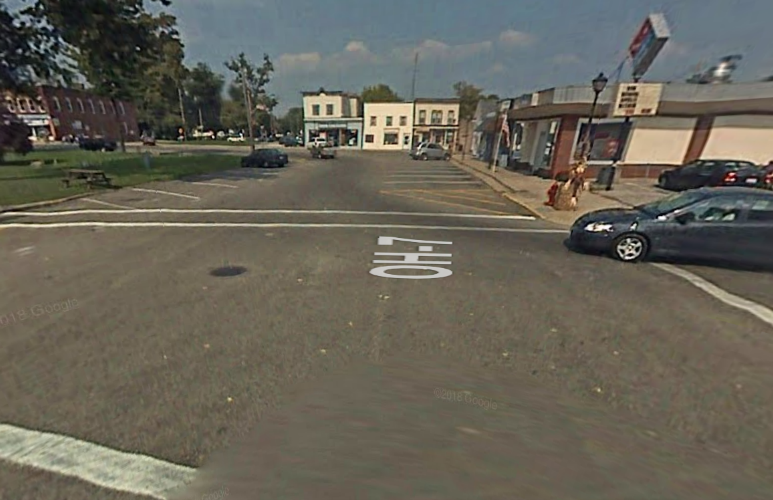
\includegraphics[width=\textwidth,keepaspectratio]{images/andover_township_14grandarmy_2007.png}
            \caption{Grand Army of the Republic Hwy: 2007
            \label{fig:andover_2007}}
        \end{subfigure}
    \end{minipage}
    \hfill
    \begin{minipage}[b]{0.49\textwidth}
        \centering
        \begin{subfigure}[b]{\textwidth}
            \centering
            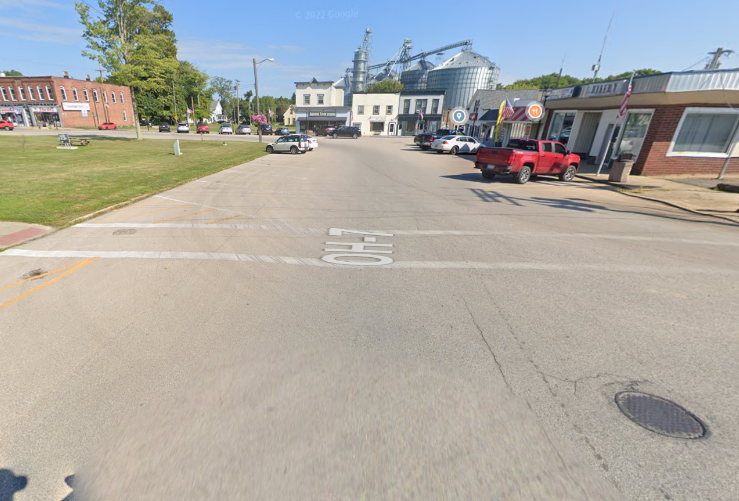
\includegraphics[width=\textwidth,keepaspectratio]{images/andover_township_14grandarmy_2022.png}
            \caption{Grand Army of the Republic Hwy: 2022}
            \label{fig:andover_2022}
        \end{subfigure}
    \end{minipage}

    \vspace{1em}

    \caption{Anover township - Road quality}
    \label{fig:rd_andover}
\end{figure}

\begin{figure}[htbp]
    \centering
    \begin{minipage}[b]{0.49\textwidth}
        \centering
        \begin{subfigure}[b]{\textwidth}
            \centering
            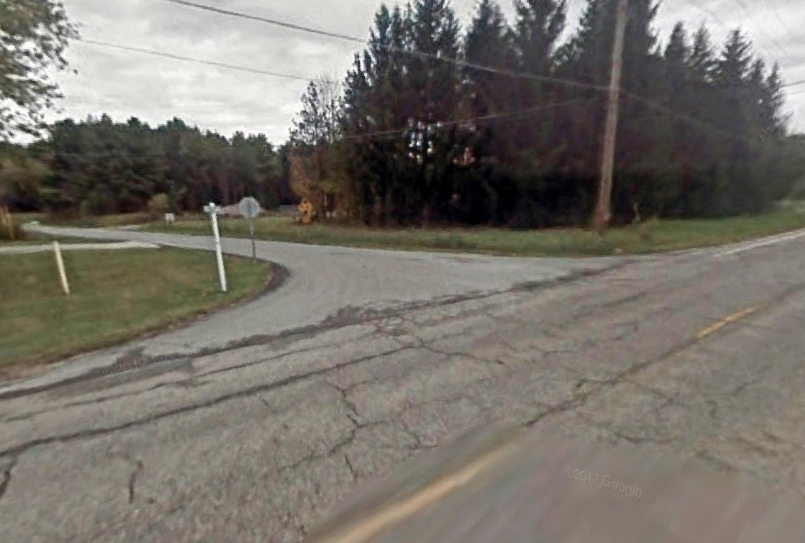
\includegraphics[width=\textwidth,keepaspectratio]{images/morgan_township_2801OH-45_2009.png}
            \caption{OH-45: 2009}
            \label{fig:morgan_oh_2009}
        \end{subfigure}
    \end{minipage}
    \hfill
    \begin{minipage}[b]{0.49\textwidth}
        \centering
        \begin{subfigure}[b]{\textwidth}
            \centering
            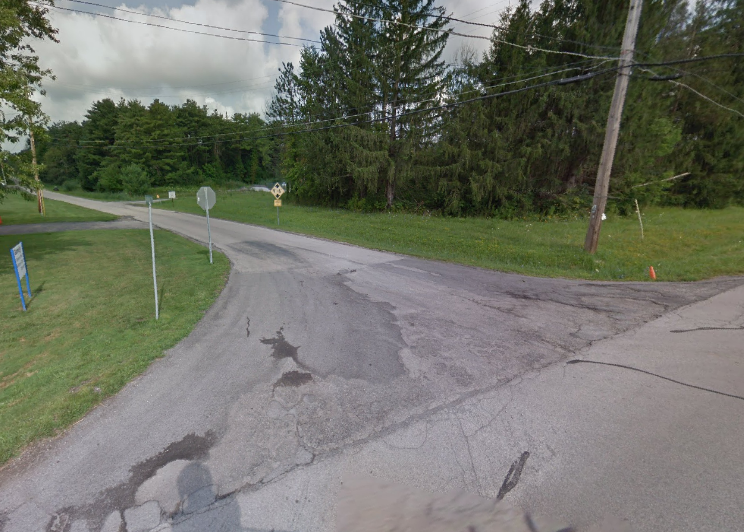
\includegraphics[width=\textwidth,keepaspectratio]{images/morgan_township_2801OH-45_2018.png}
            \caption{OH-25: 2018}
            \label{fig:morgan_oh_2018}
        \end{subfigure}
    \end{minipage}

    % \vspace{1em}

    % \begin{minipage}[b]{0.49\textwidth}
    %     \centering
    %     \begin{subfigure}[b]{\textwidth}
    %         \centering
    %         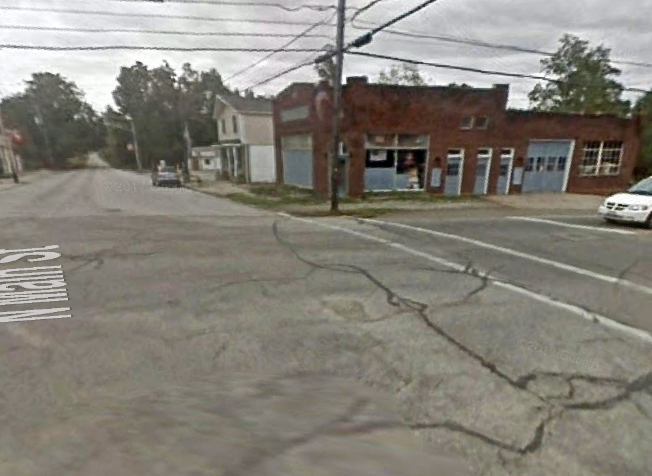
\includegraphics[width=\textwidth,keepaspectratio]{images/morgan_township_3000 W Water St_2009.png}
    %         \caption{W Water St: 2009}
    %         \label{fig:morgan_w_2009}
    %     \end{subfigure}
    % \end{minipage}
    % \hfill
    % \begin{minipage}[b]{0.49\textwidth}
    %     \centering
    %     \begin{subfigure}[b]{\textwidth}
    %         \centering
    %         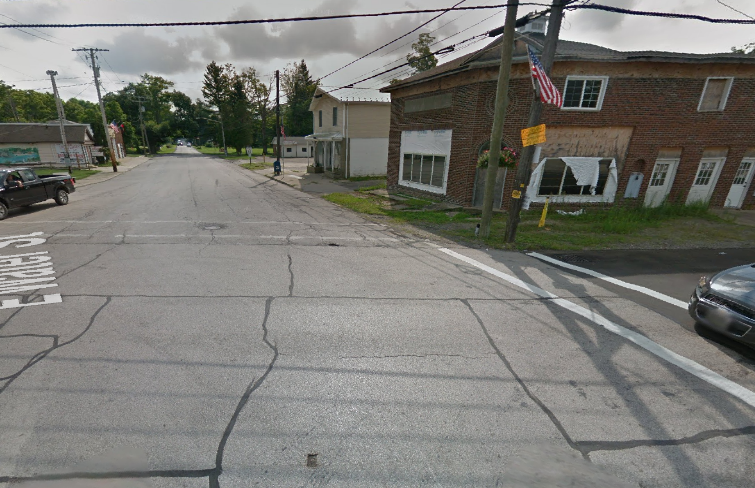
\includegraphics[width=\textwidth,keepaspectratio]{images/morgan_township_3000 W Water St_2018.png}
    %         \caption{W Water St: 2018}
    %         \label{fig:morgan_w_2018}
    %     \end{subfigure}
    % \end{minipage}    

    \caption{Morgan township - Road quality}
    \label{fig:rd_morgan}
\end{figure}

Table \ref{tab:max_renewals_cuts} shows that there are certain cities which always renew their road tax levies and other cities which often cut their renewal tax levies. Interestingly, we find two townships, Andover and Morgan, which belong to the same county of Ashtabula but exhibit very different behavior in terms of their voting patterns. Andover township passed all the road tax levies that were up for election whereas Morgan township failed to renew more than 56\% of its renewal levies. Since both the townships belong to the same county and have similar characteristics, we can effectively identify whether cutting road spending via road tax levies have a tangible impact on the quality of roads in the area. For this, we leverage Google Street Maps (GSM). Since photos of roads on GSM are time-stamped and the same area can have photos from different points in time, this feature allows us to observe the evolving condition of roads in these neighborhoods over time. For instance, we can observe the major streets of Andover township and compare them with the main streets of Morgan township. We checked whether there were any road tax renewals that took place between these available dates and then observed whether the road conditions improved, stayed the same or deteriorated during this period. Figure \ref{fig:rd_andover} shows Grand Army of the Republic Hwy, a specific hub in Andover, for periods 2007 and 2022. The road quality appears to have been maintained well over the years, indicating that consistent renewal of road tax levies contributes to sustained road infrastructure quality. In contrast, Figure \ref{fig:rd_morgan} illustrates the condition of OH-45 and W Water St in Morgan township for the years 2009 and 2018. The deterioration as well as continuation of poor road quality is evident, suggesting that the failure to renew road tax levies has a tangible negative impact on roads. The disparity in road conditions between Andover and Morgan townships may be suggestive of the broader economic implications of fiscal policy decisions at the local level, particularly how underinvestment in infrastructure can lead to tangible declines in public asset quality and potentially hinder economic growth and development.

% \clearpage

\subsection{Running Variable}

The running variable plays a critical role in regression discontinuity.  In our case it represents the proportion of votes against the renewal of a road tax levy.  A vote share of less than 50 means the tax will no longer be collected, and road funding from that particular tax levy will stop.  Other road tax levies may continue to be in effect, and funds from current expense tax levies may still be used for road maintenance.  There are 3,188 votes in our sample, 83\% of which renew the tax, and 17\% of which cut taxes and road maintenance.

We quantify the size of the cut in road spending a city faces in two ways.  First, not every city has a tax levy in effect specifically for roads, but every city has current expense tax funding.  Our mean 1.9 mill road tax represents 13.6\% of current expense funding, indicating that cities that fail to renew a road tax levy face a moderate reduction in funding.  We also investigate the drop in road expenditures by sampling financial audits of cities in our sample whose renewal tax levies fail, finding an average drop of \$218,808 in road spending one year later.  This \$218,808 drop represents a 34\% decrease in road spending.  
In our sample, the mean vote share against the tax levy is 0.38, which is essentially the same as the median of 0.36.  The standard deviation is 0.15, so that the typical levy that fails represents a little less than one standard deviation away from the mean. The Great Financial Crisis falls in the middle of our dataset, so readers might wonder if voting behavior was affected, but we find vote share the same to two decimal points during and outside the years 2008-2009. 


\subsection{Outcome Variables}

We study three different outcomes:  house prices, wages, and employment, although the most consistent set of treatment effects are for house prices.  

\subsubsection{Median Housing Price}

Our house price data comes from a CoreLogic® dataset of actual sales transaction prices in Ohio from 1995 through 2021 containing a little more than 7 million observations. The dependent variable, \textit{Median House Price}, reflects the median sale price of houses within a specific city and year. For example, for the houses sold in Delaware Township during the year 2002, the median sale price was \$205,041. We take precaution to only include arm’s-length transactions, and we restrict our attention to single-family residential structures for comparability.  The overall sample mean for the 10-year period from the time of vote considered in this study is \$166,082 in constant 2010 dollars with a standard deviation of \$372,135 which suggests presence of some outliers. Although our use of median sale price addresses outliers, our robustness check in Section 4.1.2 drops 1\% tails and re-estimates the treatment effects.  The mean for this winsorized sample is \$150,375 in constant 2010 dollars with a standard deviation of \$116,020. A staple feature of regression discontinuity studies is a graph of the outcome variable against the running variable. Figures \ref{fig:rd_hp_1} and \ref{fig:rd_hp_2} shows house prices from years $t+1$ to $t+8$ after the vote graphed against the percent of votes for the tax levy.

\begin{figure}[ht]
    \centering
    \begin{minipage}[b]{0.48\textwidth}
        \centering
        \begin{subfigure}[b]{\textwidth}
            \centering
            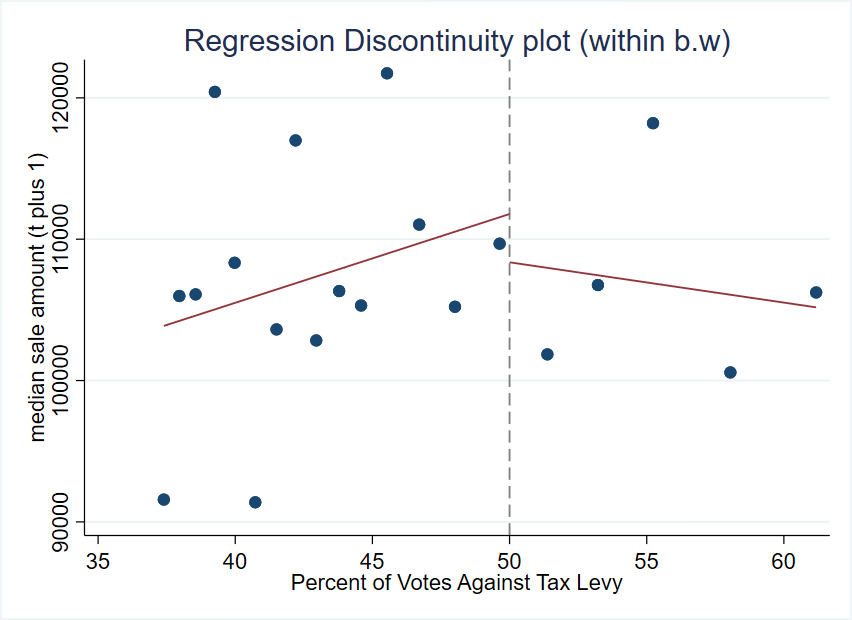
\includegraphics[width=\textwidth,keepaspectratio]{images/rd_plot_median_sale_amount_t_plus_1_tri_mserd_1_2_within.png}
            \caption{Year 1 after vote}
            \label{fig:hp_year1_after}
        \end{subfigure}
    \end{minipage}
    \hfill
    \begin{minipage}[b]{0.48\textwidth}
        \centering
        \begin{subfigure}[b]{\textwidth}
            \centering
            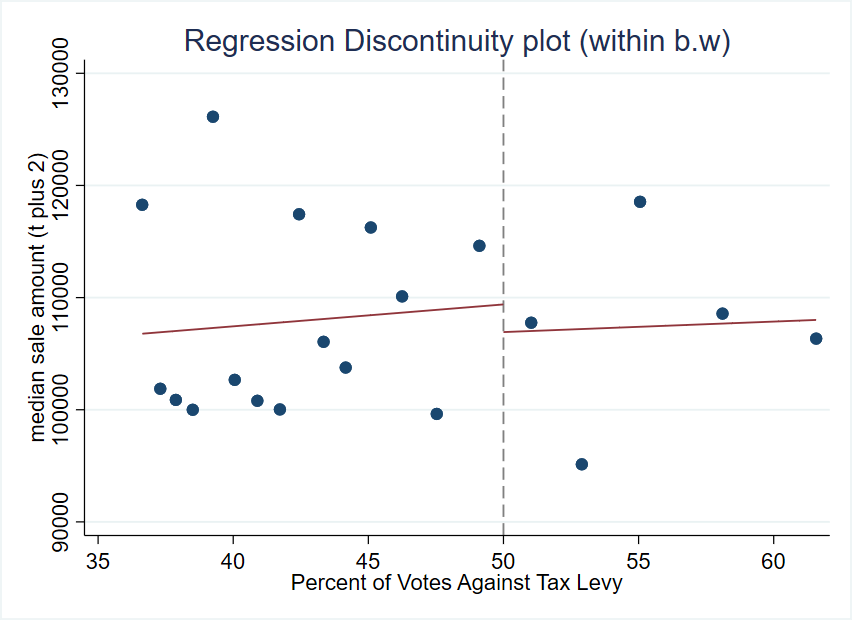
\includegraphics[width=\textwidth,keepaspectratio]{images/rd_plot_median_sale_amount_t_plus_2_tri_mserd_1_2_within.png}
            \caption{Year 2 after vote}
            \label{fig:hp_year2_after}
        \end{subfigure}
    \end{minipage}

    \vspace{1em}

    \begin{minipage}[b]{0.48\textwidth}
        \centering
        \begin{subfigure}[b]{\textwidth}
            \centering
            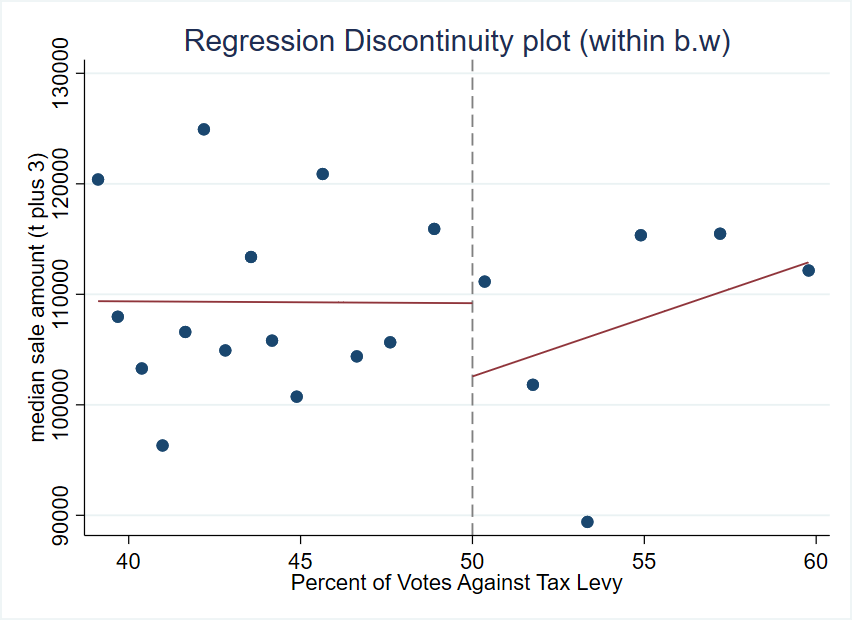
\includegraphics[width=\textwidth,keepaspectratio]{images/rd_plot_median_sale_amount_t_plus_3_tri_mserd_1_2_within.png}
            \caption{Year 3 after vote}
            \label{fig:hp_year3_after}
        \end{subfigure}
    \end{minipage}
    \hfill
    \begin{minipage}[b]{0.48\textwidth}
        \centering
        \begin{subfigure}[b]{\textwidth}
            \centering
            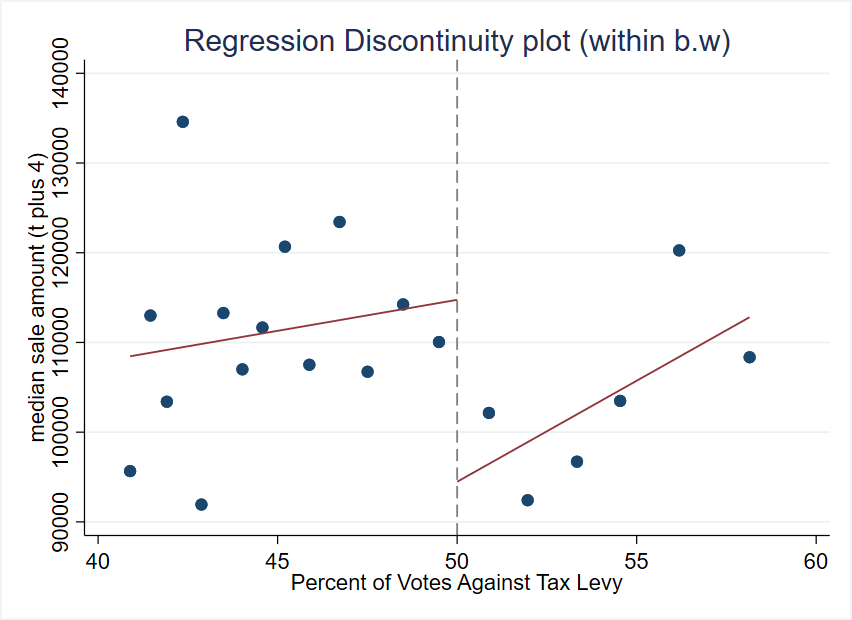
\includegraphics[width=\textwidth,keepaspectratio]{images/rd_plot_median_sale_amount_t_plus_4_tri_mserd_1_2_within.png}
            \caption{Year 4 after vote}
            \label{fig:hp_year4_after}
        \end{subfigure}
    \end{minipage}
    \caption{Median Housing Price as a function of running variable: up to year 4}
    \label{fig:rd_hp_1}
\end{figure}

\begin{figure}[ht]
    \centering
    \begin{minipage}[b]{0.48\textwidth}
        \centering
        \begin{subfigure}[b]{\textwidth}
            \centering
            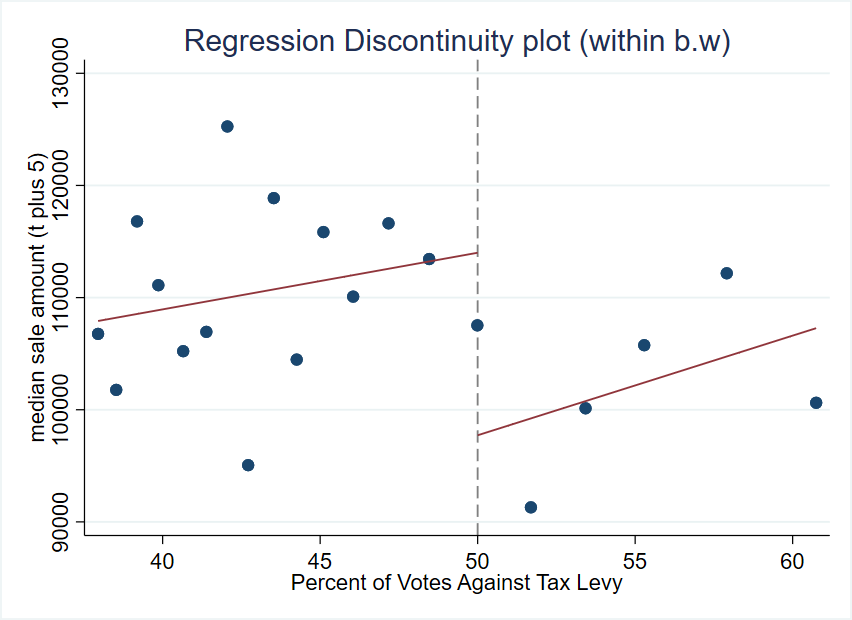
\includegraphics[width=\textwidth,keepaspectratio]{images/rd_plot_median_sale_amount_t_plus_5_tri_mserd_1_2_within.png}
            \caption{Year 5 after vote}
            \label{fig:hp_year5_after}
        \end{subfigure}
    \end{minipage}
    \hfill
    \begin{minipage}[b]{0.48\textwidth}
        \centering
        \begin{subfigure}[b]{\textwidth}
            \centering
            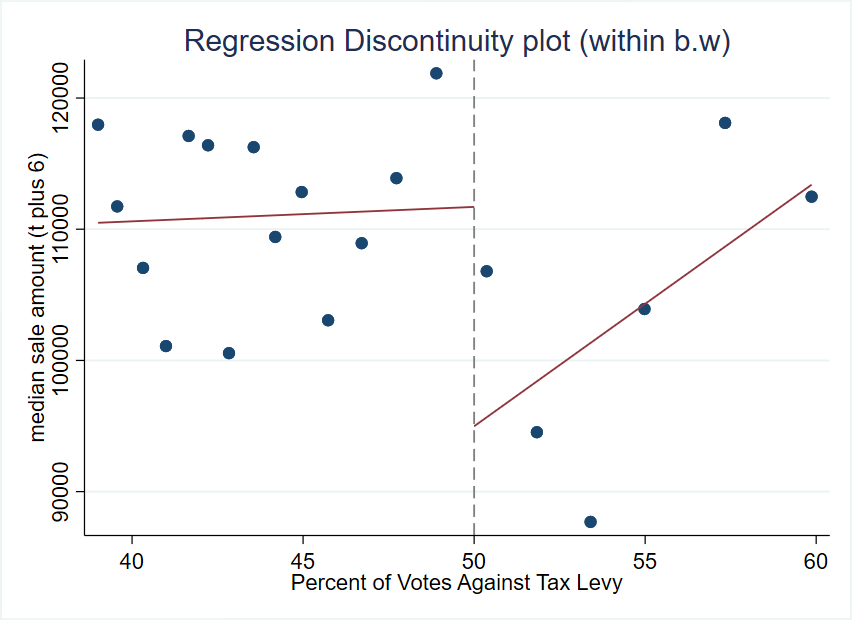
\includegraphics[width=\textwidth,keepaspectratio]{images/rd_plot_median_sale_amount_t_plus_6_tri_mserd_1_2_within.png}
            \caption{Year 6 after vote}
            \label{fig:hp_year6_after}
        \end{subfigure}
    \end{minipage}    

    \vspace{1em}

    \begin{minipage}[b]{0.48\textwidth}
        \centering
        \begin{subfigure}[b]{\textwidth}
            \centering
            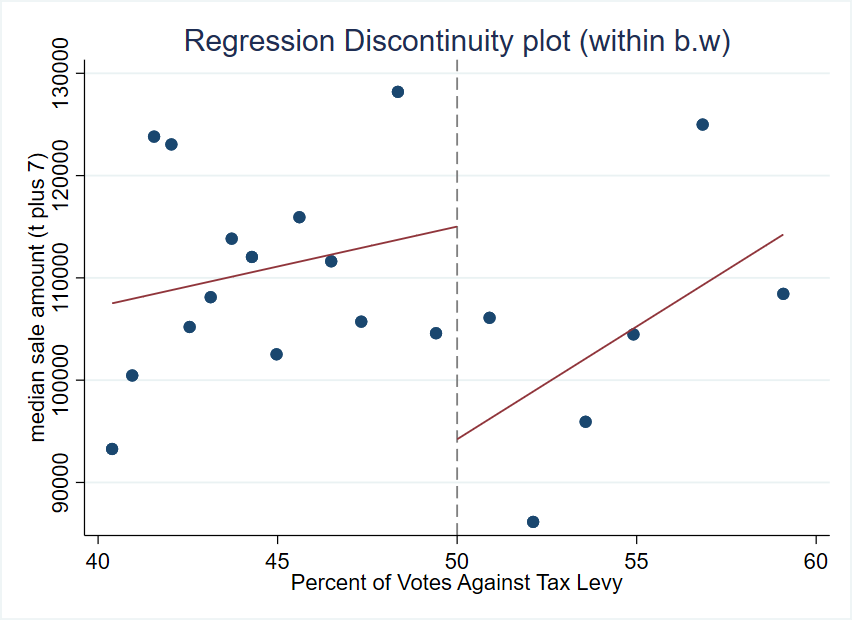
\includegraphics[width=\textwidth,keepaspectratio]{images/rd_plot_median_sale_amount_t_plus_7_tri_mserd_1_2_within.png}
            \caption{Year 7 after vote}
            \label{fig:hp_year7_after}
        \end{subfigure}
    \end{minipage}
    \hfill
    \begin{minipage}[b]{0.48\textwidth}
        \centering
        \begin{subfigure}[b]{\textwidth}
            \centering
            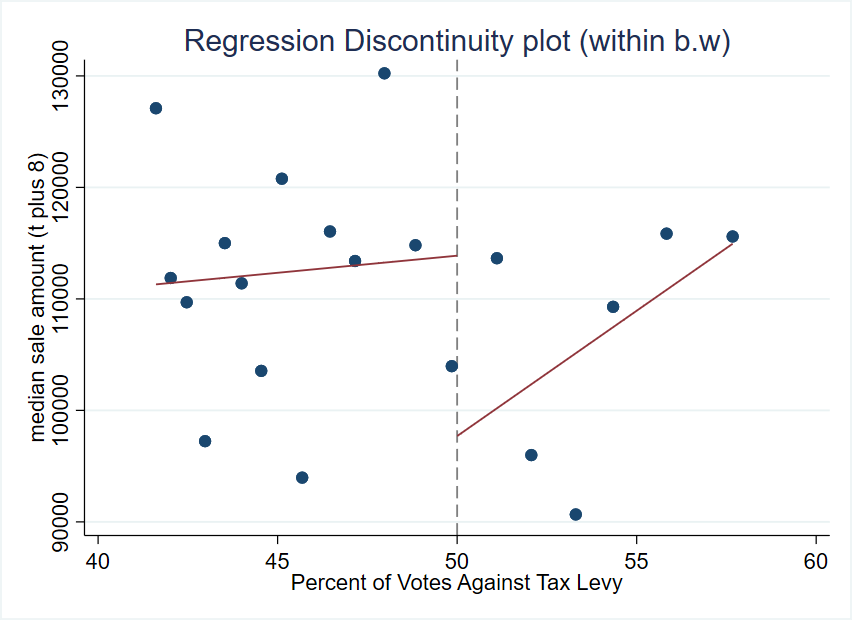
\includegraphics[width=\textwidth,keepaspectratio]{images/rd_plot_median_sale_amount_t_plus_8_tri_mserd_1_2_within.png}
            \caption{Year 8 after vote}
            \label{fig:hp_year8_after}
        \end{subfigure}
    \end{minipage}        

    \caption{Median Housing Price as a function of running variable: year 5 to year 8}
    \label{fig:rd_hp_2}
\end{figure}


Scatterplots like Figure \ref{fig:rd_hp_1} and \ref{fig:rd_hp_2}, although expected in regression discontinuity studies, should be read with caution, because the dots in the graphs do not represent actual house prices or vote shares.  A graph of actual data would illustrate a mess of dots for which no human could see a discernible pattern.  Graphing involves averaging vote shares into bins representing a narrow range of vote shares and summarizing the wide range of house prices within each bin with a single mean value.  For this reason, graphs do not necessarily track treatment effects that come from formal regression analysis using actual individual data points.  Nevertheless, the graphs in Figure \ref{fig:rd_hp_1} and \ref{fig:rd_hp_2} representing 8 years after the vote may show a discount in house prices from cutting taxes and road maintenance. Corresponding estimates and graphs for treatment effects in the full set of years $t+1$ through $t+10$ relative to the vote can be found in Figure \ref{fig:tes_gs_app} and Table \ref{tab:median_sale_amount_full} in the Appendix.

\subsubsection{Employment and Wages}

We obtain special permission from the Ohio Department of Jobs and Family Services (ODJFS) to access establishment-level data on wages and employment.  It shows total wages and the average number of employees for each quarter.  We aggregate up from quarterly to yearly values.  Each establishment has an address, which we geocode to the proper local government jurisdiction (city, village or township), and we aggregate total wages and average employment up to the local government level to match the unit of geography of the voting data. The outcome variables considered were “Average employment” and “Wages per capita”, where average employment is the average number of employees on the payroll in a particular city during a specific year, and wages per capita is aggregate total wages paid to the employees on the payroll in particular city during a year divided by average employment. Graphs of these outcome variables are available upon request.  Within the typical effective bandwidth of 14 percentage points, mean city-level employment is 1,575 for the fail levy group with a standard deviation of 3,319; and it is 1,342 with a standard deviation of 3,514 for the pass levy group the year before the vote.  

The average wage outcome we study also has similar means within the effective bandwidth the year before the vote.  For the high-poverty sample, the sample with the only significant treatment effects, mean wages in 2010 dollars are \$29,153 for the fail-levy sample with a standard deviation of 8,515; and they are \$29,968 for the pass-levy sample with a standard deviation of 7,524.

\subsection{Covariates}

Covariates can be useful in regression discontinuity studies, although they are not necessary for the identification of treatment effects.  One use of covariates is to increase the precision of treatment effect estimates.  The other is to see if cities that barely pass and fail tax levies are similar to each other like the theory of regression discontinuity says they should be. Table \ref{tab:variable_means_sd} shows covariate means for both the global sample of all votes in the data set as well as the local sample within a representative effective bandwidth of the 0.50 cutoff. The effective bandwidth displayed in Table \ref{tab:variable_means_sd} is the mean bandwidth for all the housing outcome regressions. The first columns for the global sample show similar values of characteristics between cities that renew and cut road taxes and spending, but it is the two rightmost columns that are critical for the credibility of the regression discontinuity design.   

Table \ref{tab:variable_means_sd} demonstrates the covariate balance between cities that renew their tax levies and those that do not, indicating similar demographic and economic profiles across both groups. The data, captured at the time of the vote, shows minimal differences within the effective bandwidth: the mean population differs by only 224 from a base of 5,220, and median family income varies by \$190 from a base of \$60,269, measured in 2010 U.S. dollars. Other variables, including poverty rates, single-parent household percentages, educational attainment, age distribution, and racial composition, show differences of less than one percentage point, reinforcing the comparability of the two groups.


\begin{longtable}{p{4cm}cccccc}
    \caption{Variable Means \& Standard Deviation by Tax Levy Renewal Status} \label{tab:variable_means_sd} \\
    \hline
    Variable & \multicolumn{3}{c}{Global} & \multicolumn{2}{c}{Effective} \\
    \cmidrule(lr){2-4} \cmidrule(lr){5-6}
    & Full Sample & Renewed & Cut & Renewed (Control) & Cut (Treatment) \\
    \hline
    \endfirsthead

    \multicolumn{6}{c}{{\bfseries \tablename\ \thetable{} -- continued from previous page}} \\
    \hline
    Variable & \multicolumn{3}{c}{Global} & \multicolumn{2}{c}{Effective} \\
    \cmidrule(lr){2-4} \cmidrule(lr){5-6}
    & Full Sample & Renewed & Cut & Renewed (Control) & Cut (Treatment) \\
    \hline
    \endhead

    \hline \multicolumn{6}{r}{{Continued on next page}} \\
    \endfoot

    \hline
    \endlastfoot

    \multicolumn{6}{l}{\textbf{Panel A. Covariates}} \\
    Population & 5,074 & 5,134 & 4,769 & 5,220 & 4,996 \\
               & (7,942) & (8,030) & (7,478) & (8,205) & (7,420) \\
    Poverty Rate & 0.11 & 0.11 & 0.11 & 0.11 & 0.10 \\
                 & (0.08) & (0.08) & (0.07) & (0.08) & (0.07) \\
    \% with Kids & 0.39 & 0.39 & 0.40 & 0.39 & 0.39 \\
                 & (0.08) & (0.08) & (0.08) & (0.08) & (0.07) \\
    \% Households with Children under 18 & 0.09 & 0.09 & 0.09 & 0.09 & 0.08 \\
                                         & (0.06) & (0.06) & (0.05) & (0.06) & (0.05) \\
    \% Less than High School Education & 0.16 & 0.15 & 0.18 & 0.17 & 0.18 \\
                                       & (0.11) & (0.11) & (0.10) & (0.11) & (0.09) \\
    \% Some College Education & 0.25 & 0.25 & 0.24 & 0.25 & 0.24 \\
                              & (0.06) & (0.06) & (0.06) & (0.06) & (0.07) \\
    \% Unemployment Rate & 0.05 & 0.05 & 0.05 & 0.06 & 0.05 \\
                         & (0.04) & (0.04) & (0.03) & (0.04) & (0.03) \\
    \% Renters & 0.20 & 0.20 & 0.20 & 0.20 & 0.19 \\
               & (0.11) & (0.11) & (0.10) & (0.11) & (0.09) \\
    \% White & 0.96 & 0.96 & 0.97 & 0.97 & 0.96 \\
             & (0.07) & (0.08) & (0.07) & (0.08) & (0.08) \\
    \% Black & 0.02 & 0.02 & 0.02 & 0.02 & 0.02 \\
             & (0.07) & (0.07) & (0.06) & (0.07) & (0.07) \\
    \% Married & 0.59 & 0.59 & 0.60 & 0.60 & 0.61 \\
               & (0.09) & (0.09) & (0.08) & (0.09) & (0.08) \\
    \% Separated & 0.01 & 0.01 & 0.01 & 0.01 & 0.01 \\
                 & (0.01) & (0.01) & (0.01) & (0.01) & (0.01) \\
    Income Heterogeneity Index & 0.10 & 0.10 & 0.09 & 0.09 & 0.09 \\
                               & (0.08) & (0.08) & (0.07) & (0.07) & (0.06) \\
    Median Family Income & 61,014 & 61,445 & 58,837 & 60,269 & 60,079 \\
                         & (17,694) & (18,283) & (14,177) & (15,687) & (14,143) \\
    \% Under 5 Years Old & 0.06 & 0.06 & 0.06 & 0.06 & 0.06 \\
                         & (0.02) & (0.02) & (0.02) & (0.02) & (0.02) \\
    \% Aged 5 to 17 & 0.20 & 0.20 & 0.21 & 0.20 & 0.20 \\
                    & (0.05) & (0.05) & (0.04) & (0.05) & (0.04) \\
    \% Aged 18 to 64 & 0.60 & 0.60 & 0.60 & 0.60 & 0.60 \\
                     & (0.05) & (0.05) & (0.05) & (0.05) & (0.04) \\
    \% Racial Minority & 0.04 & 0.04 & 0.03 & 0.03 & 0.04 \\
                       & (0.07) & (0.08) & (0.07) & (0.08) & (0.08) \\
    Number of Observations & 3,188 & 2,661 & 527 & 694 & 273 \\
    \\
    \multicolumn{6}{l}{\textbf{Panel B. Outcome Variables}} \\
    \textit{a) Median House Price} & & & & & \\
    t - 3 & 106,067 & 107,502 & 102,766 & 106,771 & 104,201 \\
          & (52,988) & (60,197) & (50,794) & (53,461) & (51,794) \\
    t - 2 & 105,528 & 107,211 & 101,456 & 106,207 & 103,713 \\
          & (53,242) & (60,893) & (48,438) & (54,162) & (50,786) \\
    t - 1 & 107,706 & 108,234 & 104,575 & 108,401 & 105,843 \\
          & (53,544) & (62,437) & (51,343) & (54,665) & (50,491) \\
    \textit{b) Employment} & & & & & \\
    t - 3 & 1,504 & 1,752 & 1,728 & 1,446 & 1,695 \\
          & (3,848) & (4,006) & (3,642) & (3,887) & (3,739) \\
    t - 2 & 1,429 & 1,734 & 1,680 & 1,388 & 1,562 \\
          & (3,693) & (3,978) & (3,612) & (3,769) & (3,462) \\
    t - 1 & 1,387 & 1,724 & 1,668 & 1,341 & 1,538 \\
          & (3,628) & (3,993) & (3,598) & (3,683) & (3,460) \\
    \textit{c) Wages per Capita} & & & & & \\
    t - 3 & 31,764 & 31,892 & 32,531 & 32,367 & 32,401 \\
          & (8,868) & (8,428) & (10,090) & (9,657) & (8,898) \\
    t - 2 & 31,714 & 32,083 & 32,048 & 31,571 & 32,166 \\
          & (8,630) & (8,392) & (9,224) & (8,723) & (8,372) \\
    t - 1 & 31,764 & 32,399 & 32,399 & 31,579 & 32,367 \\
          & (8,868) & (9,716) & (9,716) & (8,623) & (9,657) \\
\end{longtable}

% \begin{tablenotes}
%     \small
%     \item Notes: Panel A shows covariates used in estimating the treatment effect of failing to renew a road tax levy. Covariate means at the time of the vote are shown along with standard deviations in parentheses. The unit of observation is city-year. 'Income' is median family income in constant 2010 U.S. dollars. 'Global' refers to the full sample of city-year votes; 'Effective' refers to city-year votes within the mean estimated optimal bandwidth of 10 percentage points around the cutoff for years 1995 through 2021. The treatment group reflects cutting road funding by failing to renew the road tax levy. The control group reflects maintaining road funding by renewing the road tax levy. Panel B shows means of outcome variables for placebo years t - 3, t - 2, and t - 1.
% \end{tablenotes}


Table \ref{tab:variable_means_sd} shows that the treatment and control groups are well-balanced with respect to the covariates considered, suggesting that the groups are comparable and any observed differences in outcomes can more confidently be attributed to the treatment effect rather than to pre-existing differences.

\subsection{Testing how well the data meets the assumptions of RDD}

The assumptions of regression discontinuity are minimal compared to other identification strategies.  One is that no agent, while having some influence, may precisely assign observations to a specific value of the running variable.  In our context, it means that higher levels of government, foreign governments, or the firm that programs the voting machines may not dictate vote share for city road tax levies.  The standard way to test this assumption is to perform a density test like that of \cite{cattaneo2020simple}, which is based on the idea that a manipulating agent might cause a clustering of votes just to one side of the cutoff, with a pronounced drop-off on the other side of the cutoff.  The $p$-value of this density test is 0.98. A histogram of vote share is shown in Figure \ref{fig:running_var_hist} that graphically illustrates the lack of abrupt change in density.  

\begin{figure}[ht]
    \centering
    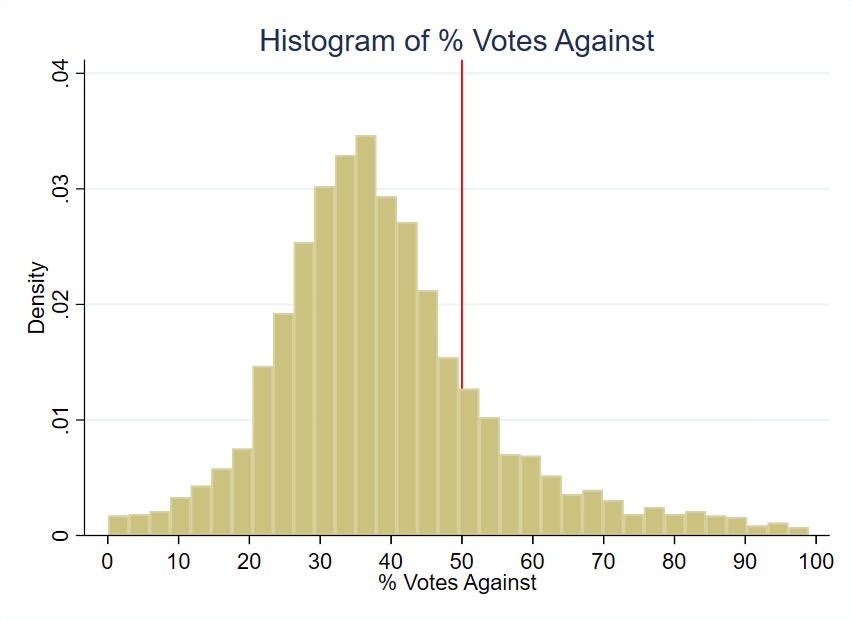
\includegraphics[width=\textwidth,keepaspectratio]{images/votes_pct_against_histogram.png}
    \caption{Histogram of Running Variable}
    \label{fig:running_var_hist}
\end{figure}

Although Table \ref{tab:variable_means_sd} shows covariate balance between sets of cities that pass and fail to renew road tax levies, covariate values could still jump from one side of the cutoff to another. A drop in education levels, for example, could cause a drop in house prices that might coincide with a change in treatment, so that what might look like a treatment effect from cutting taxes and spending might in fact be caused by lower education levels.  Graphs of covariate smoothness around the cutoff are found in the Appendix \ref{sec:appxb}. A formal way to assess covariate smoothness is to use each covariate as an outcome variable in a regression of the running variable and a treatment effect dummy. When we do so, the $p$-value of the treatment effect dummy varies from 0.13 to 0.98, indicating no statistically significant jump in covariate values. 

\section{Methodology} \label{sec:method}

We follow a model of sharp Regression Discontinuity Design (RDD), as detailed in \cite{calonico2019regression}. A formal description of the model is provided below. Let $Y_{it}$ represent the outcome variable for city, village or township $i$ at year $t$. The outcome variables we study include house prices, wages, and employment. Drawing from the Rubin causal model, we use potential outcomes notation to describe $Y_{it}(1)$ as a potential outcome variable if exposed to treatment and $Y_{it}(0)$ as the potential outcome variable in absence of treatment i.e. our control. We define treatment as failure of a city, village or township to renew its road maintenance tax levy. Let $T_{it} \in \{0,1\}$ represent cities that receive treatment (1) or not (0) based on voting at year $t$, so that our realized outcome is represented by the following equation:

$$
Y_{it} = Y_{it}(1) \times T_{it} + Y_{it}(0) \times (1-T_{it})
$$

Let $X_{it}$ be the running variable that determines whether a realized outcome variable was treated or not based on some cutoff $\underbar{x}$. In our study, the running variable is the percent of votes against the renewal tax levy and the cutoff is 50 percent. Let $Z_{it}$ be our vector of covariates and $\tau$ be our parameter of interest i.e. the treatment effect. This parameter of interest measures the causal effect of cutting road maintenance spending on different outcome variables. Under the assumption of continuity at the cutoff $\underbar{x}$, the RDD allows us to compute the average treatment effect $\tau = \mathbb{E}(Y_{it}(1) - Y_{it}(0) | X_{it} = \underbar{x})$. We employ both local polynomial and local randomization approaches to compute the estimate for $\tau$, which we call $\hat{\tau}$.

To observe the persistence of treatment effects, we develop an event study-styled estimator that tracks the outcome variable for different values in future. The regression equation takes the form -

$$
Y_{i(t+r)} = \alpha_r + T_{i(t+r)} \tau_r + X_{i(t+r)} \beta_r + T_{i(t+r)} X_{i(t+r)} \theta_r + Z_{i(t+r)} \gamma_r + \epsilon_{i(t+r)}
$$

\noindent where $r \in \{-3,-2, ..., 10 \}$, $\alpha_r$ is the intercept, $\beta_r$ is the coefficient on the running variable $X_{i(t+r)}$, $\theta_r$ is the coefficient of the interaction term, $\gamma_r$ is a vector of coefficients for covariates matrix $Z_{i(t+r)}$ and $\epsilon_{i(t+r)}$ is the idiosyncratic error term. Our parameter of interest, $\tau_r$ measures the causal effect of cutting road maintenance spending on different outcome variables for different values of $r$. We estimate the treatment effect for different values of $r$ to observe the persistence of treatment effects and consider the possibly of placebo effects. 

The above equation has been described in detail in \cite{calonico2019regression} and is called the covariate-adjusted RDD estimator. We use the bandwidth selection method described in \cite{calonico2019regression} to choose a bandwidth $h$ and then conduct a local linear polynomial regression after choosing a weighting scheme. The bandwidth $h$ determines size of the neighborhood around the cutoff $\underbar{x}$, where the neighborhood is $(\underbar{x}-h, \underbar{x}+h)$. Only observations with values of the running variable within this neighborhood are used to compute the treatment effect estimate $\hat{\tau}$ and, for a small enough neighborhood, the continuity assumption central to the RDD estimator is satisfied. The weighting scheme $k$ determines the weights of the observations within the neighborhood $(\underbar{x}-h, \underbar{x}+h)$ and is another important factor in determining $\hat{\tau}$. The most common types of weighting schemes are uniform, triangular and Epanechnikov. We use the default Mean Squared Error Regression Discontinuity (MSERD) method to compute the effective bandwidth ($h$) and bias bandwidth ($b$) for each outcome variable. This method identifies the bandwidth that minimizes the trade-off between bias and variance of the treatment effect estimate. All observations are used to estimate $h$ and $b$, but only the observations within the selected bandwidth $h$ i.e. effective observations within $h$ percentage points on either side of the 0.50 vote share cutoff are used to identify our treatment effect estimates.


\section{Results} \label{sec:results}

First, we share the results for house prices. Next, we present the results for employment and wages outcome variables.

\subsection{House Prices}

We find no significant treatment effect of changes in road taxes and funding on house prices in years $t+1$ through $t+3$ relative to the year of the vote, so we relegate these regression results to Table \ref{tab:median_sale_amount_full}.  On the other hand, Table \ref{tab:median_sale_amount} below shows the treatment effect estimates of failing a road tax levy on housing sale prices starting four years after the vote. 

\begin{table}[ht]
    \centering
    \caption{Effect on median house prices of failing to renew a road tax levy}
    \label{tab:median_sale_amount}
    \begin{tabular}{p{2cm}ccccccc}
        \hline
        year relative to vote & $t + 4$ & $t + 5$ & $t + 6$ & $t + 7$ & $t + 8$ & $t + 9$ & $t + 10$ \\
        \hline
        Treatment effect & -19,535 & -21,531 & -16,994 & -16,691 & -23,323 & -30,620 & -16,411 \\
        Standard error & (9,289) & (9,147) & (7,558) & (7,357) & (9,449) & (9,586) & (9,342) \\
        Effective bandwidth ($h$) & 8.9 & 12.1 & 14.1 & 14.0 & 8.2 & 8.2 & 8.3 \\
        Bias bandwidth ($b$) & 15.4 & 20.0 & 24.1 & 24.2 & 15.5 & 16.3 & 17.5 \\
        Effective Observations & 714 & 1,020 & 1,182 & 1,127 & 593 & 584 & 557 \\
        Total Observations & 2,618 & 2,535 & 2,442 & 2,328 & 2,204 & 2,119 & 2,022 \\
        \hline
    \end{tabular}
    \begin{tablenotes}
        \small
        \item Outcome is median house price in constant 2010 U.S. dollars. Unit of observation is the city-year, so a treatment effect of -\$19,535 means that four years after the vote, cities that failed to renew road taxes and its associated spending have houses that sell for \$19,535 less than cities that vote to renew road taxes and spending. Treatment effects for years prior to $t + 4$ are statistically insignificant at 5\% level; full results shown in Table \ref{tab:median_sale_amount_full}. The regressions include covariates related to the demographics and socioeconomic factors of the cities, drawn from Table \ref{tab:variable_means_sd}.
    \end{tablenotes}
\end{table}

Each treatment effect estimate represents the discount in median sale price for cities that cut road taxes and spending in the years after voting on a road tax levy relative to otherwise similar cities that renew the taxes. For instance, the treatment effect for the $t + 4$ outcome variable is -19,535.  This means that four years after the vote, the median house sale price is \$19,535 lower in cities that fail to renew their road tax levy, relative to cities that vote to renew their road taxes and spending. Treatment effect estimates for years 4 through 9 after the vote are statistically significant in Table \ref{tab:median_sale_amount} as the $p$-values are below the canonical 0.05 threshold.  The estimate for year $t + 10$ has a smaller estimate and is only significant at the 10\% level, suggesting that the effect of tax and service cuts on house prices may peter out ten years after the vote. Overall, we find an average reduction of \$20,729 in median house price from years $t+4$ to $t+10$ for houses in cities that vote to cut road tax levies representing 12\% of house value.

\begin{figure}[htbp]
    \centering
    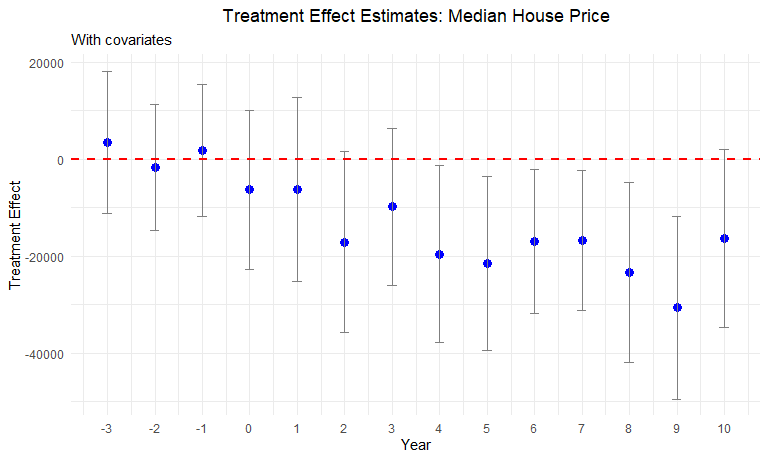
\includegraphics[width=\textwidth,keepaspectratio]{images/tes_gs.png}
    \caption{Effect plot for Median Housing Price}
    \label{fig:tes_hp}
\end{figure}

Figure \ref{fig:tes_hp} provides an event-study plot that summarizes the treatment effects for each time period. In the graph, we include placebo years up to 3 years before the treatment to show that the median housing prices are statistically identical for cities above and below the threshold prior to the treatment. Each blue dot represents the treatment effect estimate for that year and the bar around it represents the 95\% confidence interval for that estimate. For year 0, which is the year of the vote, we see a slight decrease in the estimate. However, this effect is not statistically significant, as evidenced by the confidence interval containing the null effect. Up to year 3, we observe that the treatment effect estimates are fairly close to zero, and the confidence interval overlaps with zero. As stated previously and shown in Table \ref{tab:median_sale_amount}, we start to see a sizable increase in treatment effect from year 4 onwards and continue to observe it through year 9 after the vote. 

\subsubsection{Heterogeneity Analysis} We show the results of our heterogeneity analysis, where we explore the differential impact of cutting road maintenance spending on house prices based on urban vs rural neighborhoods, the size of the tax levy and housing price quantiles.

\vskip 0.5cm

\textbf{Urban vs Rural neighborhoods}: We perform heterogeneity analysis to assess whether different types of neighborhoods and differing size of tax levies result in a differential impact on the housing prices. We first compare urban and rural areas in Ohio. We consider two different ways to define a city as urban:  one including only urbanized areas and another one including both urban areas and urbanized clusters. The event study plot in Figure 6 shows this result. 

\begin{figure}[htbp]
    \centering
    % 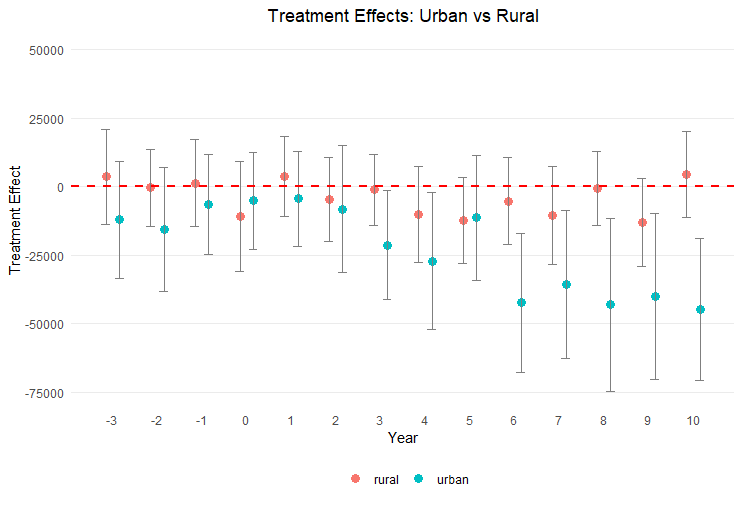
\includegraphics[width=\textwidth,keepaspectratio]{images/tes_covs_ua_new.png}
    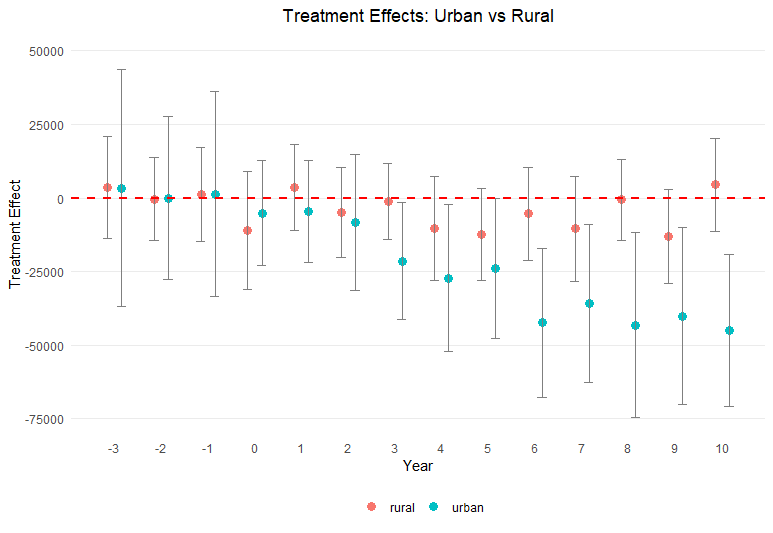
\includegraphics[width=\textwidth,keepaspectratio]{images/tes_covs_ua_clean.png}    
    \caption{Median Housing Price in Urban and Rural Areas}
    \label{fig:tes_covs_ua}
\end{figure}

As shown by Figure \ref{fig:tes_covs_ua}, we do not find any significant differences in housing prices after a renewal tax levy fails to pass for rural areas. On the other hand, we do find a statistically significant decline in housing prices in urban areas starting six years after voting. The standard errors are somewhat smaller for the rural estimates due to a larger number of observations. The difference in point estimates between urban and rural areas may stem from differences in housing supply elasticity (Brasington 2002). Overall, we find that housing prices decrease by \$25,825 on average over the decade after cutting road maintenance tax levies in urban areas. 

\vskip 1cm

\textbf{Tax magnitude}: We check whether the treatment effect is greater for bigger tax levies than smaller tax levies. For this analysis, we split the tax levies based on the millage of a tax levy that is voted upon, where one mill is one tenth of one percent. Mean millage in our dataset is 1.9. We split the data into two parts: small tax levies $\le$ 1.9 mills and large tax levies $>$ 1.9 mills. We do not identify a consistent statistically significant difference in treatment effects between smaller and larger tax levies, suggesting a lack of dose-response. Figure \ref{fig:tes_covs_size} illustrates this result.

\begin{figure}[htbp]
    \centering
    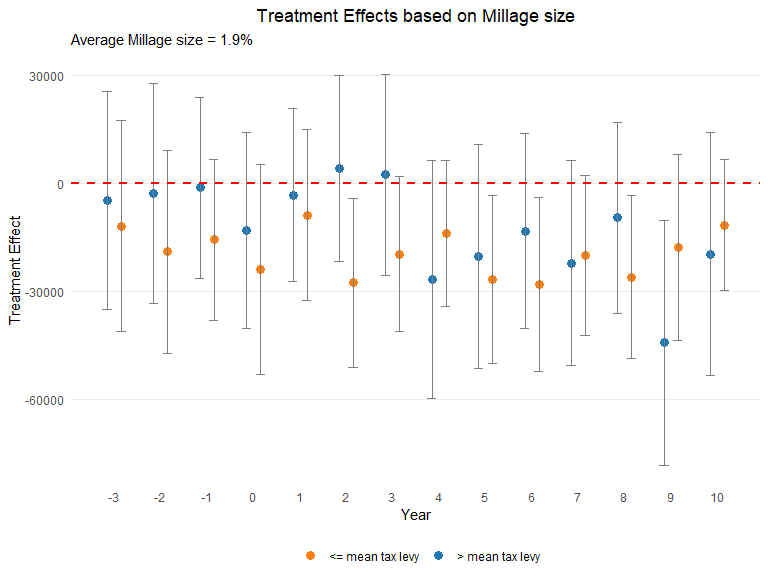
\includegraphics[width=\textwidth,keepaspectratio]{images/tes_size.png}
    \caption{Median Housing Price based on Millage size}
    \label{fig:tes_covs_size}
\end{figure}

All the years before the reduction in road spending have treatment effect estimates with confidence intervals containing zero. Starting in year $t+2$, we observe statistically significant treatment effects in some years after the vote such as year 5, 6 and 8 that show a for tax levies with millage size equal to or below the mean. However, we do not see a consistent decrease in housing prices. Hence, we conclude that the decrease in housing prices of cities that fail to maintain their roads does not vary significantly based on the size of the tax levy.

\vskip 1cm

\textbf{RDD Quantile Estimation}: We further analyze our results by estimating quantile-level treatment effects, as suggested by Frandsen et al (2012), to study how the treatment’s impact varies at different quantiles of the outcome variable. 

\begin{table}[ht]
    \hspace{-1cm}
    % \centering
    \caption{Quantile-level Treatment Effects of Cutting Road Spending on Median House Prices}
    \label{tab:quantile_tes}
    \begin{tabular}{p{1.5cm}ccccccc}
        \hline
        Percentile & $t + 4$ & $t + 5$ & $t + 6$ & $t + 7$ & $t + 8$ & $t + 9$ & $t + 10$ \\
        \hline
        10\% & -6,433 & -22,570 & -9,602 & -12,984 & -11,217 & -6,569 & -1,326 \\
        & (9,364) & (9,065) & (9,205) & (8,420) & (9,136) & (10,809) & (8,793) \\
        20\% & -5,400 & -15,070 & 4,014 & -14,682 & -15,040 & -3,228 & 624 \\
        & (9,983) & (9,886) & (7,443) & (8,502) & (8,160) & (10,435) & (8,509) \\
        70\% & -21,760 & -11,171 & -38,082 & -36,685 & -21,356 & -25,605 & -18,600 \\
        & (12,333) & (11,806) & (12,835) & (12,163) & (12,218) & (13,984) & (9,872) \\
        80\% & -28,478 & -16,379 & -38,460 & -37,470 & -28,950 & -27,800 & -18,658 \\
        & (13,343) & (11,404) & (18,623) & (12,169) & (12,507) & (12,421) & (11,808) \\
        90\% & -51,470 & -34,604 & -38,510 & -27,039 & -29,010 & -49,093 & -36,662 \\
        & (18,409) & (15,837) & (22,194) & (16,308) & (16,640) & (14,498) & (19,110) \\
        \hline
    \end{tabular}
    \begin{tablenotes}
        \small
        \item The outcome is median house price in constant 2010 U.S. dollars. The unit of observation is the city-year, so a treatment effect of -\$28,478 means that at the 80th percentile of house prices four years after the vote, cities that fail to renew road taxes and its associated spending have houses that sell for \$28,478 less than cities that vote to renew road taxes and spending. The regressions include covariates related to the demographics and socioeconomic factors of the cities, drawn from Table \ref{tab:variable_means_sd}.
    \end{tablenotes}
\end{table}

\begin{figure}[htbp]
    \centering
    % 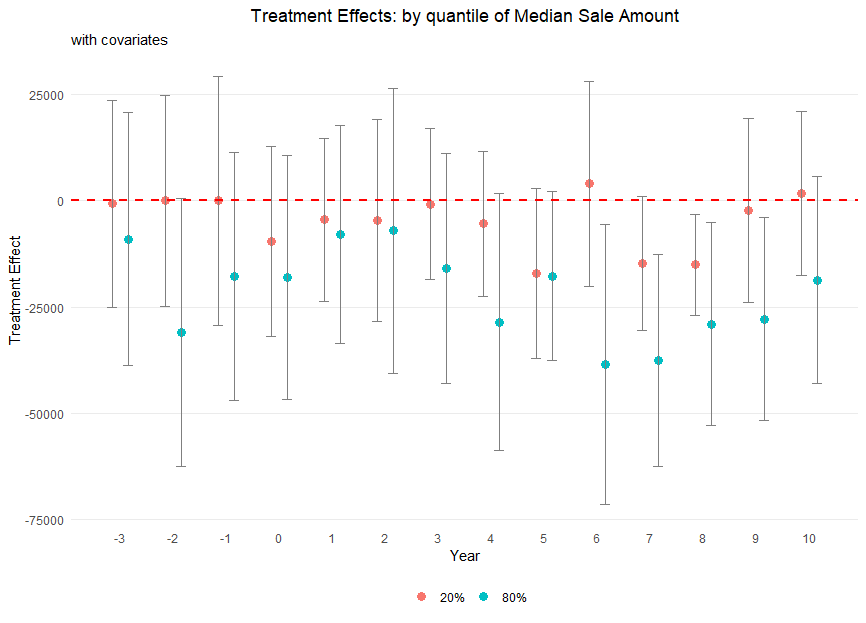
\includegraphics[width=\textwidth,keepaspectratio]{images/tes_qte_covs.png}
    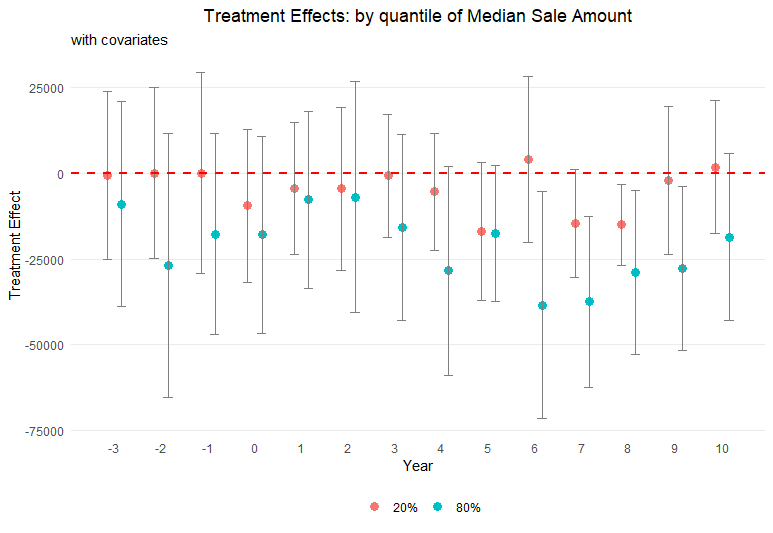
\includegraphics[width=\textwidth,keepaspectratio]{images/tes_qte.png}    
    \caption{Median Housing Price based on Quantiles: 20\% and 80\%}
    \label{fig:tes_qte_covs}
\end{figure}

Table \ref{tab:quantile_tes} shows the treatment effect heterogeneity of cutting road spending on high and low quantiles of median house prices. The top percentiles consistently exhibit a statistically significant decline in house sale prices, beginning in year 6 after the reduction in road spending. In contrast, the lower percentiles do not demonstrate a consistent treatment effect. This suggests a differential impact, where higher-valued properties are more sensitive to road disrepair than lower-valued houses. Figure \ref{fig:tes_qte_covs} contrasts the treatment effects of the 20th and 80th percentiles of home sale prices in an effect plot to highlight this differential impact of reduction in road maintenance spending.

\subsubsection{Robustness Tests} We conduct several robustness tests to ensure the validity of our results. We test the sensitivity of our results to different bandwidths, covariates, and functional forms. We also check for the presence of pre-trends and perform a placebo test to confirm the validity of our RDD.

\vskip 0.5cm

\textbf{Removing contradictory observations}: In this test, we focus on ensuring the independence and exogeneity of our dataset, a critical aspect in assessing the impact of renewal tax levies on housing prices. An additional concern is the potential bias introduced by tax levies for additional money that might pass after renewal tax levy decisions.
To address this concern, we exclude observations from our analysis if a tax levy for additional funding is introduced and passed within a ten-year period following a renewal tax levy vote. This approach is premised on the notion that the introduction of new funding through additional levies could confound the effects of decreased road taxes on housing prices. 
For example, consider a scenario where a city votes on a renewal tax levy in the year 2000. If that city subsequently introduces and passes a tax levy for additional road spending in 2004, we exclude all votes for that city from 2005 through 2010. This exclusion ensures that the effect on house prices from the 2000 vote are captured for uncontaminated years but not for years after 2004 when the effect of additional road taxes may counteract the drop in tax money from the year 2000 vote. It allows us to isolate and examine the pure impact of the drop in funding from failing renewal levies on housing prices. 

\begin{table}[ht]
    \centering
    \caption{Effect on Median Sale Amount of Failing to Renew a Road Tax Levy}
    \label{tab:uncontaminated}
    \begin{tabular}{p{2.8cm}ccccccc}
        \hline
        year relative to vote & $t + 4$ & $t + 5$ & $t + 6$ & $t + 7$ & $t + 8$ & $t + 9$ & $t + 10$ \\
        \hline
        Treatment effect & -21,819 & -16,308 & -13,850 & -15,944 & -18,443 & -29,298 & -19,179 \\
        standard error & (11,271) & (7,489) & (8,161) & (8,186) & (8,591) & (8,342) & (10,120) \\
        Effective bandwidth (h) & 7.7 & 7.4 & 14.7 & 10.5 & 9.4 & 6.2 & 8.9 \\
        Bias bandwidth (b) & 13.6 & 17.8 & 24.5 & 19.0 & 18.4 & 13.3 & 18.2 \\
        Effective Observations & 538 & 512 & 1,086 & 680 & 584 & 347 & 492 \\
        Total Observations & 2,390 & 2,273 & 2,147 & 2,016 & 1,889 & 1,786 & 1,665 \\
        \hline
    \end{tabular}
    \begin{tablenotes}
        \small
        \item The outcome is median house price in constant 2010 U.S. dollars. The unit of observation is the city-year, so a treatment effect of -\$21,819 means that four years after the vote, cities that fail to renew road taxes and its associated spending have houses that sell for \$21,819 less than cities that vote to renew road taxes and spending. The regressions include covariates related to the demographics and socioeconomic factors of the cities, drawn from Table \ref{tab:variable_means_sd}.
    \end{tablenotes}
\end{table}

Upon implementing this data filtration, we observe that the treatment effect of the renewal levies on housing prices, measured from $t+1$ to $t+10$, remains largely consistent with our initial findings. This consistency in treatment effect, despite the exclusion of potentially confounding data, lends further credence to our results. The standard errors increase slightly due to reduction in sample size caused by the aforementioned data filtration process. 

\textbf{Placebo cutoffs}: In our primary analysis, the pivotal threshold for the vote share running variable is 50\%, indicating whether a renewal levy passes or fails.  Although we find significant treatment effects using this 50\% threshold, it could be random jumps in the data rather than cutting road taxes and funding that are responsible for the significant estimates.  To this end we conduct a series of placebo tests using alternative cutoffs: 30\%, 40\%, 60\%, and 70\%. Table \ref{tab:placebo_cutoffs} below summarizes the results from the placebo cutoffs analysis. 

\begin{table}[ht]
    \centering
    \caption{Robust Treatment Effect Estimate for Placebo Cutoffs}
    \label{tab:placebo_cutoffs}
    \begin{tabular}{p{2cm}cccc}
        \hline
        Years after vote & 30\% & 40\% & 60\% & 70\% \\
        \hline
        $t + 4$ & -2,540 & 7,037 & -4,037 & -43,670 \\
        & (8,473) & (6,993) & (10,961) & (21,452) \\
        $t + 5$ & -1,376 & -15,672 & -1,740 & 12,263 \\
        & (9,554) & (20,892) & (12,588) & (19,392) \\
        $t + 6$ & 10,589 & 9,476 & -13,479 & -617 \\
        & (8,894) & (7,721) & (13,661) & (18,438) \\
        $t + 7$ & 5,086 & 2,952 & -21,731 & -21,204 \\
        & (10,447) & (7,898) & (11,519) & (18,330) \\
        $t + 8$ & 9,900 & 11,821 & -11,014 & -37,686 \\
        & (10,745) & (8,241) & (12,460) & (15,717) \\
        $t + 9$ & 14,361 & 9,904 & -20,057 & -9,340 \\
        & (9,624) & (7,935) & (11,975) & (17,731) \\
        $t + 10$ & 12,147 & -25,540 & -13,828 & -16,358 \\
        & (13,649) & (31,460) & (10,267) & (21,396) \\
        \hline
    \end{tabular}
    \begin{tablenotes}
        \small
        \item Robust treatment effect estimate for placebo cutoffs as per the estimator from \cite{calonico2017rdrobust}. The unit of observation is city-year level. Standard errors are shown in parentheses below each estimate.
    \end{tablenotes}
\end{table}

Table \ref{tab:placebo_cutoffs} does not show consistently significant treatment effects for any of the placebo cutoffs for our parameter of interest. This absence of significance at thresholds other than the true 50\% reinforces the idea that the effects we observe at the 50\% mark are not a mere coincidence or a result of random variation in the data, but are indeed attributable to the dynamics surrounding the passing or failing of renewal tax levies. 

\textbf{Winsorization}: The debate over whether to include or exclude outliers continues, with some research suggesting that trimming outliers does not improve mean squared error (e.g., Bollinger and Chandra, 2005).  We now drop the 1\% tails to help curtail the influence of outliers. The overall sample mean after dropping 1\% tails is \$144,268 in constant 2010 dollars with a standard deviation of \$109,624. After performing this winsorization step, we re-estimate the treatment effect of failing to renew a road tax levy on housing outcome variables. The results from this estimation process are summarized in Figure \ref{fig:tes_g_w} below:

\begin{figure}[htbp]
    \centering
    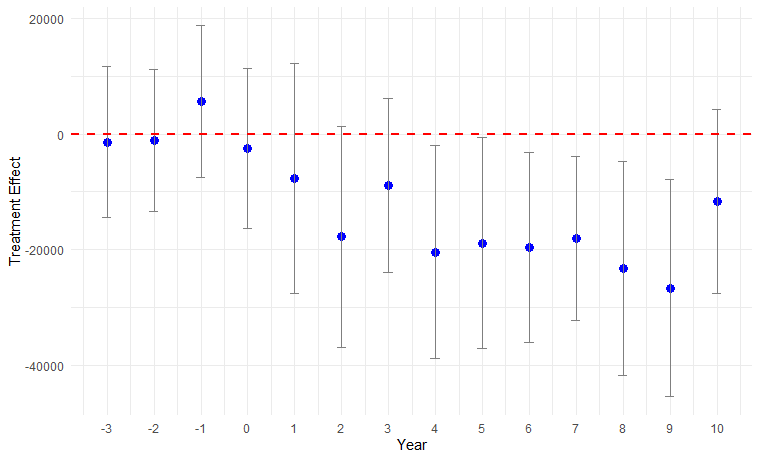
\includegraphics[width=\textwidth,keepaspectratio]{images/tes_g_w.png}
    \caption{Median Housing Price after 1\% Winsorization}
    \label{fig:tes_g_w}
\end{figure}

The treatment effect estimates with winsorization mimic those from our baseline regression results qualitatively and quantitatively.

\subsection{Employment} \label{sec:employment}

We next see if cutting road taxes and spending causes a change in employment in years after the vote. Employment is the average number of workers in a city in a year, which comes from monthly employment data per establishment as provided by ODJFS.  The regressions take the same form as explained in Section \ref{sec:method}.  The full set of null results is shown in Appendix \ref{sec:appxa} Table \ref{tab:average_employment} and Table \ref{tab:log_average_employment}.

On the other hand, when we examine an interaction term between poverty and treatment, there is a consistent pattern of significant results.  The estimator of \cite{calonico2019regression} cannot handle interaction terms, but our first step is to use it to establish an optimal bandwidth of the running variable.  We then omit all votes outside the optimal effective bandwidth.  We then create an interaction term between the treatment dummy $T_{i(t+r)}$ and Poverty Rate.  We then regress employment as a function of the running variable, the treatment effect dummy, the interaction term, and the covariates Median Family Income, \% Aged 5 to 17, and \% Less than High School Education.  For certain years, the covariates \% Unemployment Rate, \% Under 5 Years Old, \% Less than High School Education, and \% Some College Education were helpful in achieving precise estimates of the treatment effect. Table \ref{tab:treatment_dummy_poverty} summarizes the results of our experiment. 
 
\begin{table}[ht]
    \centering
    \caption{Effect of cutting road spending on Employment by Poverty Rate}
    \label{tab:treatment_dummy_poverty}
    \begin{tabular}{p{2cm}cc}
        \hline
        Year after Vote & Treatment Dummy Estimate & Treatment Dummy  Poverty Rate Estimate ($p$-value) \\
        \hline
        $t - 3$ & 498 (0.46) & -2,526 (0.49) \\
        $t - 2$ & 768 (0.22) & -3,769 (0.31) \\
        $t - 1$ & 833 (0.17) & -3,649 (0.31) \\
        $t + 1$ & 1,039 (0.08) & -9,941 (0.02) \\
        $t + 2$ & 1,231 (0.03) & -7,995 (0.04) \\
        $t + 3$ & 849 (0.18) & -8,742 (0.03) \\
        $t + 4$ & 1,050 (0.10) & -10,197 (0.02) \\
        $t + 5$ & 1,279 (0.05) & -10,478 (0.02) \\
        $t + 6$ & 1,327 (0.04) & -10,483 (0.02) \\
        $t + 7$ & 1,473 (0.03) & -11,599 (0.02) \\
        $t + 8$ & 1,374 (0.04) & -11,073 (0.02) \\
        $t + 9$ & 1,528 (0.03) & -12,694 (0.02) \\
        $t + 10$ & 1,435 (0.04) & -13,202 (0.02) \\
        \hline
    \end{tabular}
    \begin{tablenotes}
        \small
        \item Estimates shown with $p$-values in parentheses below. Number of observations ranges from 565 to 722. Regressions of outcome variable Employment for optimal bandwidth estimate h = 14. Regressors include Vote Share, Treatment Dummy, Treatment Dummy  Poverty Rate, Median Family Income, \% Aged 5 to 17, and \% Less than High School Education for all years. Regression for year $t + 4$ adds \% Unemployment Rate and \% Some College Education, $t + 8$ adds \% Some College Education, the covariates for $t + 2$ are \% High School Education Only, \% Renters, and \% Under 5 Years Old, to improve the precision of the estimates.
    \end{tablenotes}
\end{table}

For the first year after the vote, the interaction term is negative with a $p$-value of 0.02, but the treatment effect is only significant at the 10\% level of significance, for a joint significance of 0.06.  However, starting with the second year after the vote and continuing through all successive years that we test--ten years after the vote--we find a consistent pattern of a positive treatment effect dummy with a negative interaction term.  The average magnitude of the estimates shows that, for cities with Poverty Rate greater than 0.11, cutting road taxes and the associated services causes lower employment, relative to cities that renew road maintenance tax levies. 

The poverty rate of 0.11 is about the 65th percentile of poverty, suggesting that high-poverty cities that renew road tax levies have better employment outcomes than those that cut road maintenance.  We evaluate the magnitude of the effect with the estimates achieved in year 4 after the vote.  For a marginal increase in the poverty rate to 12\%, renewing road maintenance taxes preserves 174 jobs on average relative to cities that cut, which represents an 11\% preservation of jobs.

\subsection{Wages}

We now investigate wages, the other outcome variable provided by ODJFS.  The raw data contains the total dollar amount of wages paid to employees by each firm in each quarter from year 2006 to 2020.  We average the quarterly data up to yearly values and convert nominal dollars to constant 2010 dollars.  We sum the firm-level data to the appropriate city, village, or township and divide by the number of workers to get average yearly wages earned by a worker in each municipality.  We find a better fit when the natural log of average wages is used, rather than a linear term, and we find a local linear functional form fits the data better than a quadratic form (adjusted mean squared error of 9.4m vs. 12.7m).

We find no effect of cutting road taxes and services on wages for the full sample.  Regression results are shown in Table \ref{tab:total_wages} and Table \ref{tab:log_total_wages}.  Section \ref{sec:employment} found an effect on employment in high-poverty cities, and the wages outcome corroborates this story. When we restrict attention to the cities with high levels of poverty—above 14\%, which represents the 75th percentile of poverty—we find that renewing road tax levies causes higher wages.  Covariate smoothness results are provided in Appendix \ref{sec:appxb}, covariate balance for this restricted sample is shown in Table \ref{tab:covariate_means_wage}, and regression results are shown in Table \ref{tab:wages_per_worker} below. 

\begin{table}[ht]
    \centering
    \caption{Effect of Failing to Renew a Road Tax Levy on Wages per Worker}
    \label{tab:wages_per_worker}
    \begin{tabular}{p{2.8cm}ccccccc}
        \hline
        year relative to vote & $t + 4$ & $t + 5$ & $t + 6$ & $t + 7$ & $t + 8$ & $t + 9$ & $t + 10$ \\
        \hline
        Treatment effect & -0.23 & -0.18 & -0.22 & -0.14 & -0.15 & -0.12 & -0.05 \\
        standard error & 0.11 & 0.04 & 0.01 & 0.10 & 0.11 & 0.09 & 0.48 \\
        Effective bandwidth (h) & 0.07 & 0.07 & 0.06 & 0.06 & 0.06 & 0.06 & 0.09 \\
        Bias bandwidth (b) & 0.12 & 0.13 & 0.12 & 0.12 & 0.12 & 0.12 & 0.19 \\
        Effective Observations & 77 & 76 & 80 & 67 & 67 & 60 & 102 \\
        Total Observations & 401 & 385 & 367 & 350 & 337 & 319 & 306 \\
        \hline
    \end{tabular}
    \begin{tablenotes}
        \small 
        \item Outcome is the natural log of mean wages per employee in a city in constant 2010 U.S. dollars. Unit of observation is the city-year, so a treatment effect of -0.23 means that four years after the vote, high-poverty cities that fail to renew road taxes and its associated spending have 23\% lower wages than high-poverty cities that vote to renew road taxes and spending. Regressions use covariates in Table \ref{tab:wages_per_worker} representing economic and demographic characteristics of the city from the American Community Survey (ACS).
    \end{tablenotes}
\end{table}

\begin{figure}[htbp]
    \centering
    % 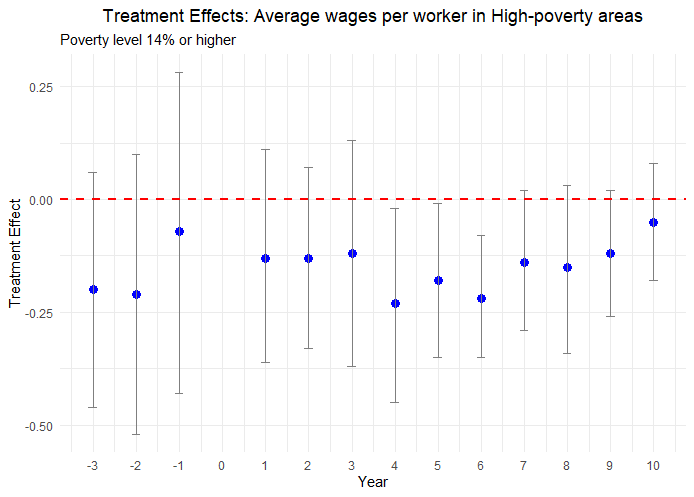
\includegraphics[width=\textwidth,keepaspectratio]{images/tes_wages_per_emp_hp.png}
    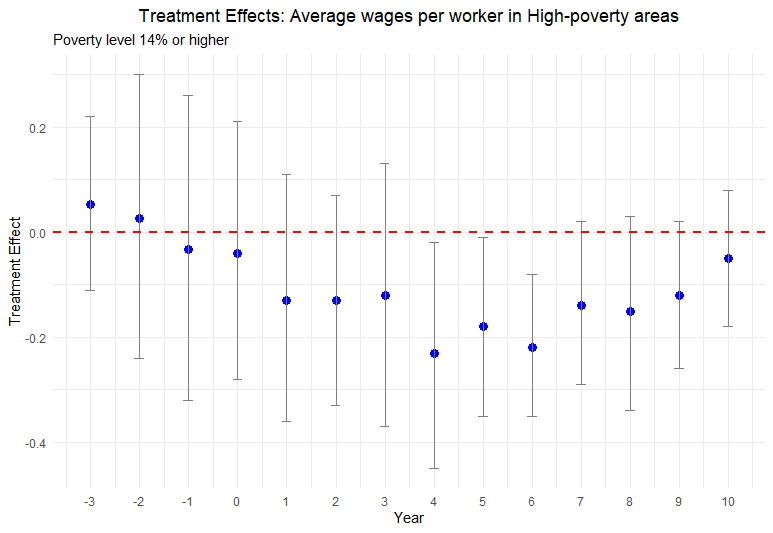
\includegraphics[width=\textwidth,keepaspectratio]{images/tes_high_pov.png}    
    \caption{Effect plot: Wages per Worker in High-Poverty Cities}
    \label{fig:tes_g_emp_hp}
\end{figure}

Significant treatment effects begin four years after the vote—later than results for the employment outcome but consistent with the house price outcome results—and continue pretty consistently through the ninth year after the vote, at least at the 10\% level of significance.  The average treatment effect suggests that high-poverty cities that renew road tax levies have 17.8\% higher wages than comparable high-poverty cities that vote to cut road maintenance taxes.  The policy implications of these results are pretty clear: road maintenance matters for wages in high-poverty areas of Ohio.  This finding is also consistent with the consensus of the literature on the effect of infrastructure investment in developing nations, which also feature high levels of poverty.

\section{Mechanisms} \label{sec:mech}

Initially, we discussed the limitations of road infrastructure papers, one of which is pinpointing a mechanism of action. \cite{currier2023} studies road roughness, finding an elasticity of speed with respect to road roughness between -0.14 and -0.30 depending on the methodology.  It also finds worse road roughness in places with lower incomes, higher racial minority fraction, and towns closer to city centers. A survey it conducts finds that towns repave only a small fraction of roads that need it, and that towns spend a lot more on resurfacing roads than other types of maintenance.

We suggest that road maintenance probably primarily affects aesthetics and productivity.  For example, the house price effects we document reflect how pretty the roads are to look at and the savings to damage to the cars that use the roads, like decreased wear on suspension, struts, shock absorbers, and damage to rims and tires. The effects we document on employment and wages in high-poverty cities are potentially driven by productivity, acting through travel time, although car damage could be involved as well:  to poorer households, car maintenance represents a high proportion of disposable income, so businesses could conceivably have to pay compensating wage differentials to induce workers to commute through poorly maintained roads. 

In Table \ref{tab:max_renewals_cuts}, we identified several cities that habitually vote against renewing road maintenance.  We traveled to one of these cities, the village of Waynesville, to investigate the condition of the roads.  While the main arteries were in satisfactory condition, most of the other roads were challenged.  Appendix \ref{sec:appxc} shows photos we took of the streets. Most were plastered with tar strips, the cheapest way to cover over cracks.  A surprising number of roads had one lane blocked for eventual road construction.  Sizeable potholes went unrepaired.  Despite the numerous problems with the roads, a police officer told us, “You should have seen the roads before!”. 

The clearest mechanism for the wage and employment outcomes is through productivity like transportation costs, commuting times, and damage to vehicles.  Some transportation studies go to great lengths to isolate one mechanism of action on house prices, but in the end the effect combines several influences like noise, crime, fatalities, car damage and travel time that are hard to disentangle.  \cite{currier2023} finds that rough roads decrease travel speed so that the cost of driving on rough roads is about 43\% higher than the cost of travel time alone, accounting for part of the house price effects we note. But our lack of wage and employment findings for the overall sample suggest that the effects of decreased road spending on house prices is probably not predominantly driven by productivity through commuting and transportation costs. We suggest that decreased attractiveness of poorly maintained roads is a ‘driving’ mechanism of our findings. Aesthetics are visible to all who use the roads, and the lagged effect on house prices is consistent with the time it might take for decreased maintenance to noticeably reducing the attractiveness of the roads. The photos we present also suggest decreased road maintenance leads to uglier roads.


\section{Conclusion} \label{sec:conclusion}

A great deal of research has studied the effect of new roads on economic outcomes like house prices, wages, and employment, especially in developing nations, providing valuable policy insights and spurring development initiatives like China’s Belt and Road Initiative and India’s Bharatmala project.  However, the endogeneity of road placement makes it difficult to identify economic effects. We study existing roads to help get around this source of confounding effects. There are many more existing roads than newly-constructed roads, especially in developed economies like the one we study, making our study especially relevant to policymakers. We study more than 3,000 votes by cities, villages, and townships in Ohio to renew maintenance spending on existing roads. We use sharp regression discontinuity to identify the effects of average treatment on the treated.  We find an average 34\% cut in road maintenance spending reduces housing sale prices by about 12\%. We find no anticipation effects, unlike \cite{beenstock2016hedonic} and \cite{diao2017spatial}, but we find statistically significant effects starting four years after funding cuts and persisting through at least the ninth year.  The effects are driven by urban rather than rural areas. We find a lack of dose-response for the size of the reduction in funding, but we find larger house price reductions for more expensive houses than for cheaper houses.  

Consistent with \cite{dalenberg1995effects} and \cite{gibbons2019new}, we cannot link road maintenance spending cuts to changes in employment or wages for our overall sample.  On the other hand, we find effects for high-poverty cities.  When the poverty rate increases by one percentage point, renewing road spending preserves 174 jobs relative to high–poverty cities that cut spending, for an 11\% difference in employment.  The effects start two years after treatment and persists through all ten years we test.  High-poverty cities (those above the 75th percentile of poverty) that cut road spending have 17.8\% lower wages than otherwise similar cities that maintain road spending. Our findings suggest that policymakers should carefully consider the long-term economic impacts of cutting road maintenance spending. While immediate budgetary savings may be appealing, the long-term costs in terms of reduced property values and economic activity, particularly in high-poverty areas, may outweigh these short-term benefits. 

 Future research could extend the regression discontinuity identification strategy we employ to other geographies, using vote share as a running variable for places that vote on road spending, or using time as a running variable for cities that directly change road spending without a referendum. Future research could also shift away from studying votes to maintain spending toward studying votes to increase road spending, although the endogeneity of choosing when to propose such a referendum makes identification more challenging.




\bibliographystyle{aea}
\bibliography{aej_references}

\pagebreak

\appendix
\section{Appendix A: Additional Treatment Effects Tables \& Effect Plots} \label{sec:appxa}

\subsection{Full set of Treatment Effects for Housing Prices}

The full set of treatment effects provided in Table \ref{tab:median_sale_amount_full} support Table \ref{tab:median_sale_amount} which provides treatment effects for the housing price outcome variable in the main body of the paper. These treatment effects are estimated using a regression model that controls for various factors.

\begin{table}[htbp]
    \centering
    \caption{Full set of estimates - Median Housing Price}
    \label{tab:median_sale_amount_full}
    \begin{tabular}{p{3cm}cccc}
        \hline
        \textbf{Year relative to vote} & \textbf{Estimate} & \textbf{Standard error} & \textbf{p-value} & \textbf{Confidence interval} \\
        \hline
        $t - 3$  & 3,468   & 7,465  & 0.642  & [-11,164, 18,099] \\
        $t - 2$  & -1,703  & 6,617  & 0.797  & [-14,673, 11,267] \\
        $t - 1$  & 1,784   & 6,950  & 0.797  & [-11,838, 15,407] \\
        $t + 1$ & -6,197  & 9,662  & 0.521  & [-25,134, 12,741] \\
        $t + 2$ & -17,059 & 9,518  & 0.073  & [-35,715, 1,597] \\
        $t + 3$ & -9,823  & 8,244  & 0.233  & [-25,981, 6,335] \\
        $t + 4$ & -19,535 & 9,289  & 0.035  & [-37,741, -1,329] \\
        $t + 5$ & -21,531 & 9,147  & 0.019  & [-39,459, -3,604] \\
        $t + 6$ & -16,994 & 7,558  & 0.025  & [-31,809, -2,180] \\
        $t + 7$ & -16,991 & 7,357  & 0.023  & [-31,111, -2,272] \\
        $t + 8$ & -23,323 & 9,449  & 0.014  & [-41,842, -4,803] \\
        $t + 9$ & -30,620 & 9,586  & 0.001  & [-49,408, -11,833] \\
        $t + 10$ & -16,411 & 9,342  & 0.079  & [-34,721, 1,898] \\
        \hline
    \end{tabular}
    \begin{tablenotes}
        \small
        \item Supplements Table \ref{tab:median_sale_amount} in text. Full set of treatment effect estimates of renewing road tax levies relative to cutting road tax levies from 3 years before the vote to 10 years after the vote. Covariates from Table \ref{tab:variable_means_sd} used in all regressions. Outcome is median house price in constant 2010 U.S. dollars. Unit of observation is the city-year. A treatment effect of -\$19,535 means that four years after the vote, cities that vote to cut road taxes and its associated spending have houses that sell for \$19,535 less than cities that vote to renew road taxes and spending.
    \end{tablenotes}
\end{table}

\begin{figure}[htbp]
    \centering
    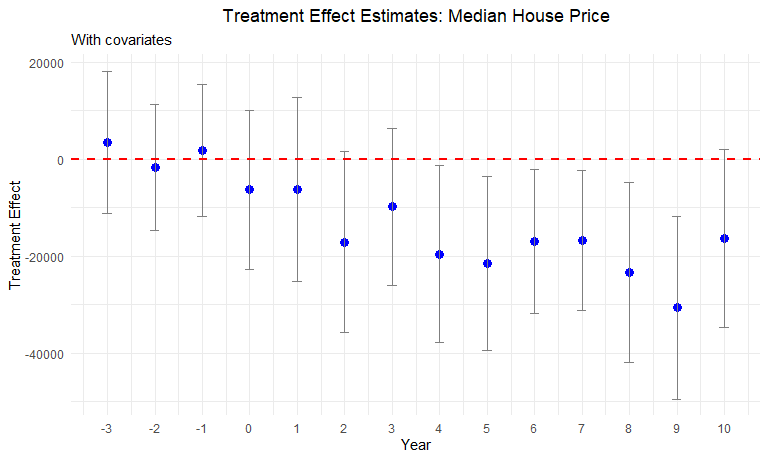
\includegraphics[width=\textwidth,keepaspectratio]{images/tes_gs.png}
    \caption{Event Study - Median Housing Price}
    \label{fig:tes_gs_app}
\end{figure}

\clearpage

\subsection{Full set of Treatment Effects for employment outcome variable}

The full set of treatment effects for the employment outcome variable for the full sample of cities have been provided below.

\begin{table}[htbp]
    \centering
    \caption{Full set of estimates - Average Employment}
    \label{tab:average_employment}
    \begin{tabular}{lcccc}
        \hline
        Year relative to vote & Estimate & Standard error & p-value & Confidence interval \\
        \hline
        $t - 3$  & 489   & 444  & 0.270  & [-380, 1359] \\
        $t - 2$  & 449   & 391  & 0.251  & [-317, 1215] \\
        $t - 1$  & 429   & 373  & 0.249  & [-301, 1160] \\
        $t + 1$ & 400   & 347  & 0.250  & [-281, 1080] \\
        $t + 2$ & 173   & 295  & 0.558  & [-406, 752] \\
        $t + 3$ & 68    & 313  & 0.827  & [-545, 682] \\
        $t + 4$ & -24   & 319  & 0.939  & [-650, 601] \\
        $t + 5$ & -100  & 343  & 0.771  & [-772, 572] \\
        $t + 6$ & -357  & 324  & 0.271  & [-993, 278] \\
        $t + 7$ & -384  & 304  & 0.206  & [-980, 211] \\
        $t + 8$ & -281  & 311  & 0.366  & [-891, 329] \\
        $t + 9$ & -237  & 350  & 0.497  & [-922, 448] \\
        $t + 10$ & -406  & 372  & 0.275  & [-1135, 323] \\
        \hline
    \end{tabular}
    \begin{tablenotes}
        \small
        \item Full set of estimates of the treatment effect on average employment for areas renewing versus cutting road tax levies, from 3 years before to 10 years after the vote.
    \end{tablenotes}
\end{table}



\begin{figure}[htbp]
    \centering
    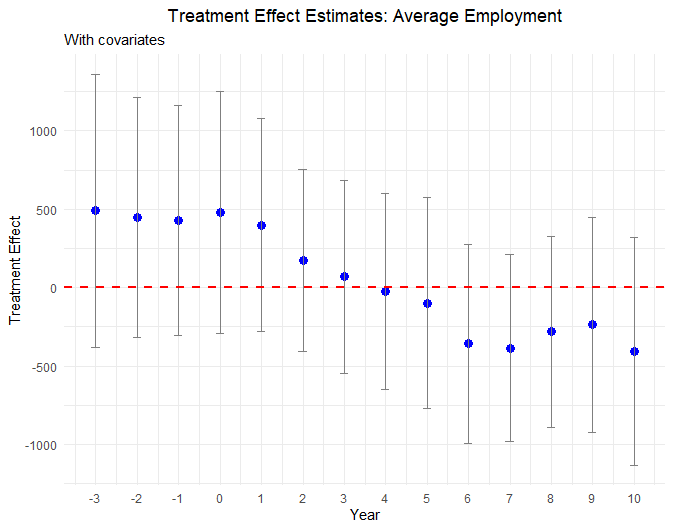
\includegraphics[width=\textwidth,keepaspectratio]{images/tes_emp.png}
    \caption{Effect plot: Average Employment}
    \label{fig:tes_gs_app}
\end{figure}

\begin{table}[htbp]
    \centering
    \caption{Full set of estimates - Log Average Employment}
    \label{tab:log_average_employment}
    \begin{tabular}{p{3cm}cccc}
        \hline
        Year relative to vote & estimate & Standard error & p-value & Confidence interval \\
        \hline
        $t - 3$  & 0.640  & 0.438  & 0.144  & [-0.218, 1.497] \\
        $t - 2$  & 0.688  & 0.392  & 0.079  & [-0.079, 1.456] \\
        $t - 1$  & 0.641  & 0.385  & 0.096  & [-0.114, 1.397] \\
        $t + 1$ & 0.308  & 0.342  & 0.368  & [-0.363, 0.98] \\
        $t + 2$ & 0.336  & 0.304  & 0.270  & [-0.261, 0.933] \\
        $t + 3$ & 0.297  & 0.285  & 0.297  & [-0.261, 0.855] \\
        $t + 4$ & 0.201  & 0.283  & 0.478  & [-0.354, 0.756] \\
        $t + 5$ & 0.235  & 0.270  & 0.385  & [-0.295, 0.765] \\
        $t + 6$ & 0.040  & 0.236  & 0.865  & [-0.422, 0.503] \\
        $t + 7$ & 0.004  & 0.238  & 0.987  & [-0.462, 0.47] \\
        $t + 8$ & -0.077 & 0.233  & 0.741  & [-0.535, 0.38] \\
        $t + 9$ & -0.094 & 0.240  & 0.696  & [-0.564, 0.377] \\
        $t + 10$ & -0.008 & 0.281  & 0.977  & [-0.56, 0.543] \\
        \hline
    \end{tabular}
    \begin{tablenotes}
        \small
        \item Full set of estimates of the treatment effect on log average employment for areas renewing versus cutting road tax levies, from 3 years before to 10 years after the vote.
    \end{tablenotes}
\end{table}

\begin{figure}[htbp]
    \centering
    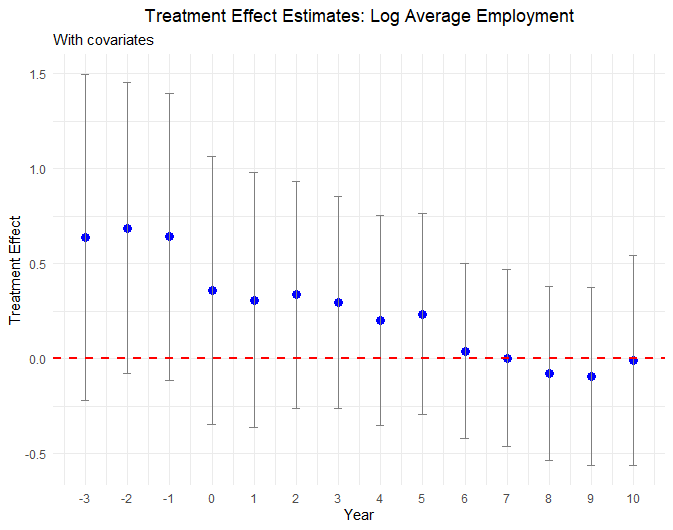
\includegraphics[width=\textwidth,keepaspectratio]{images/tes_ln_emp.png}
    \caption{Effect plot: Log Average Employment}
    \label{fig:tes_ln_emp}
\end{figure}

\clearpage

\subsection{Full set of Treatment Effects for wage outcome variable}

\begin{table}[htbp]
    \centering
    \caption{Full set of estimates - Total Wages}
    \label{tab:total_wages}
    \begin{tabular}{p{2cm}cccc}
        \hline
        Year relative to vote & Estimate & Standard error & p-value & Confidence interval \\
        \hline
        $t - 3$  & 24,989,152   & 20,849,660   & 0.231  & [-15,876,182, 65,854,486] \\
        $t - 2$  & 21,441,310   & 19,889,330   & 0.281  & [-17,541,777, 60,424,398] \\
        $t - 1$  & 19,881,825   & 19,361,782   & 0.304  & [-18,067,267, 57,830,917] \\
        $t + 1$ & 19,192,209   & 18,280,413   & 0.294  & [-16,637,400, 55,021,819] \\
        $t + 2$ & 13,929,445   & 14,858,316   & 0.349  & [-15,192,855, 43,051,744] \\
        $t + 3$ & 8,703,249    & 15,217,865   & 0.567  & [-21,123,766, 38,530,263] \\
        $t + 4$ & 4,588,179    & 15,209,473   & 0.763  & [-25,222,389, 34,398,747] \\
        $t + 5$ & 1,451,493    & 15,943,802   & 0.927  & [-29,798,358, 32,701,345] \\
        $t + 6$ & -9,929,705   & 11,649,814   & 0.394  & [-32,763,341, 12,903,931] \\
        $t + 7$ & -11,342,970  & 10,518,262   & 0.281  & [-31,958,764, 9,272,824] \\
        $t + 8$ & -8,616,720   & 10,709,258   & 0.421  & [-29,606,866, 12,373,426] \\
        $t + 9$ & -6,319,035   & 12,894,791   & 0.624  & [-31,592,825, 18,954,755] \\
        $t + 10$ & -10,837,202 & 13,975,637   & 0.438  & [-38,229,451, 16,555,046] \\
        \hline
    \end{tabular}
    \begin{tablenotes}
        \small
        \item Full set of estimates of the treatment effect on total wages for areas renewing versus cutting road tax levies, from 3 years before to 10 years after the vote.
    \end{tablenotes}
\end{table}

\begin{figure}[htbp]
    \centering
    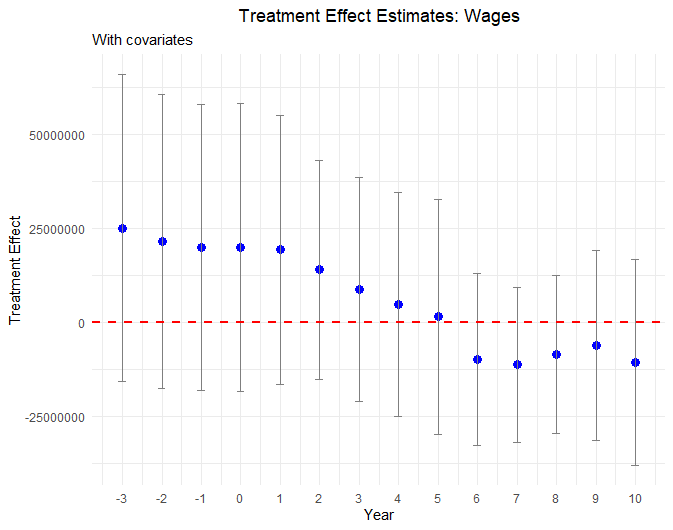
\includegraphics[width=\textwidth,keepaspectratio]{images/tes_wages.png}
    \caption{Effect plot: Wages}
    \label{fig:tes_wages}
\end{figure}


\begin{table}[htbp]
    \centering
    \caption{Full set of estimates - Log Total Wages}
    \label{tab:log_total_wages}
    \begin{tabular}{p{3cm}cccc}
        \hline
        Year relative to vote & Estimate & Standard error & p-value & Confidence interval \\
        \hline
        $t - 3$  & 0.636  & 0.496  & 0.200  & [-0.336, 1.609] \\
        $t - 2$  & 0.747  & 0.438  & 0.088  & [-0.111, 1.606] \\
        $t - 1$  & 0.740  & 0.442  & 0.094  & [-0.126, 1.605] \\
        $t + 1$ & 0.364  & 0.393  & 0.354  & [-0.406, 1.134] \\
        $t + 2$ & 0.369  & 0.348  & 0.289  & [-0.313, 1.051] \\
        $t + 3$ & 0.389  & 0.328  & 0.235  & [-0.253, 1.032] \\
        $t + 4$ & 0.230  & 0.330  & 0.485  & [-0.417, 0.877] \\
        $t + 5$ & 0.295  & 0.306  & 0.334  & [-0.304, 0.894] \\
        $t + 6$ & 0.049  & 0.262  & 0.851  & [-0.465, 0.564] \\
        $t + 7$ & 0.049  & 0.269  & 0.855  & [-0.478, 0.576] \\
        $t + 8$ & -0.031 & 0.258  & 0.905  & [-0.537, 0.475] \\
        $t + 9$ & -0.063 & 0.264  & 0.811  & [-0.58, 0.454] \\
        $t + 10$ & 0.026  & 0.306  & 0.932  & [-0.573, 0.625] \\
        \hline
    \end{tabular}
    \begin{tablenotes}
        \small
        \item Full set of estimates of the treatment effect on log total wages for areas renewing versus cutting road tax levies, from 3 years before to 10 years after the vote.
    \end{tablenotes}
\end{table}

\begin{figure}[htbp]
    \centering
    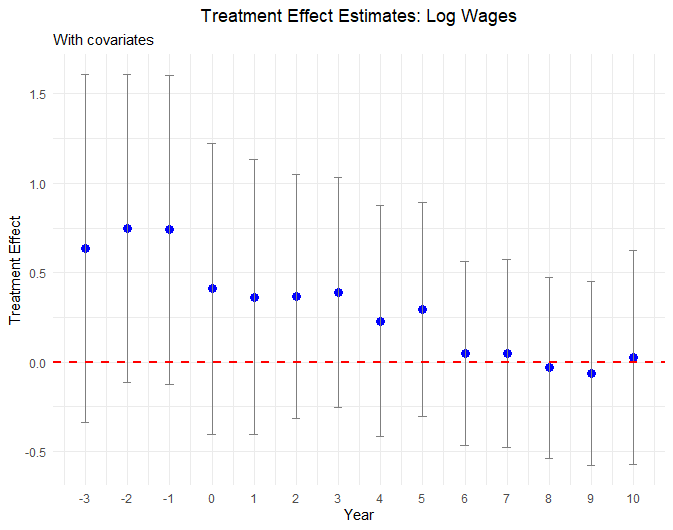
\includegraphics[width=\textwidth,keepaspectratio]{images/tes_ln_wages.png}
    \caption{Effect plot: Log Wages}
    \label{fig:tes_ln_wages}
\end{figure}

% \subsection{Outcome vs Running variable plots for years after Treatment}

\clearpage

\section{Appendix B: Additional Robustness Tests} \label{sec:appxb}

\subsection{Covariate Smoothness Plots}

\begin{figure}[ht]
    \centering
    \begin{minipage}[b]{0.48\textwidth}
        \centering
        \begin{subfigure}[b]{\textwidth}
            \centering
            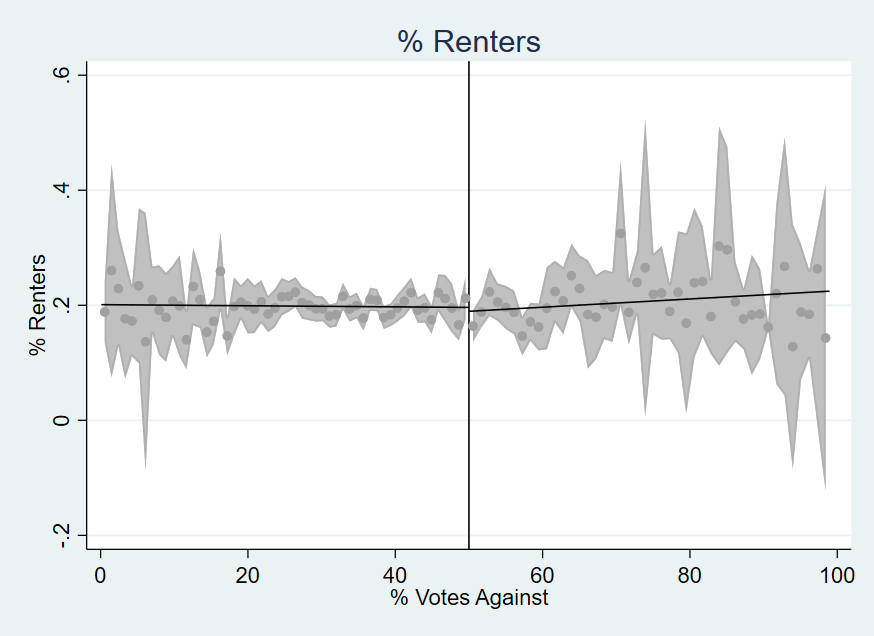
\includegraphics[width=\textwidth,keepaspectratio]{images/cov_smoothness_pctrent.png}
            % \caption{Year 1 after vote}
            \label{fig:pctrent_sm}
        \end{subfigure}
    \end{minipage}
    \hfill
    \begin{minipage}[b]{0.48\textwidth}
        \centering
        \begin{subfigure}[b]{\textwidth}
            \centering
            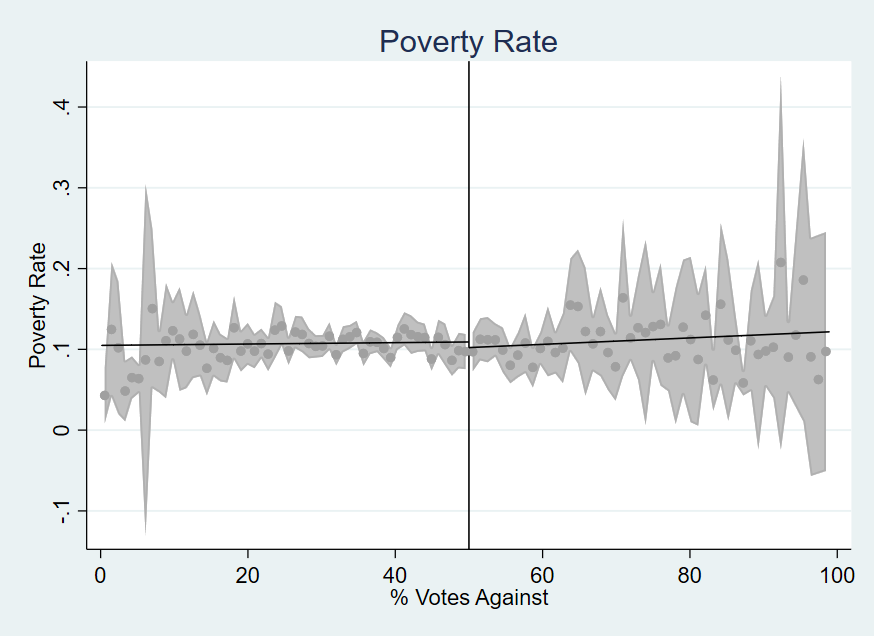
\includegraphics[width=\textwidth,keepaspectratio]{images/cov_smoothness_poverty.png}
            % \caption{Poverty Rate}
            \label{fig:poverty_sm}
        \end{subfigure}
    \end{minipage}

    \vspace{1em}

    \begin{minipage}[b]{0.48\textwidth}
        \centering
        \begin{subfigure}[b]{\textwidth}
            \centering
            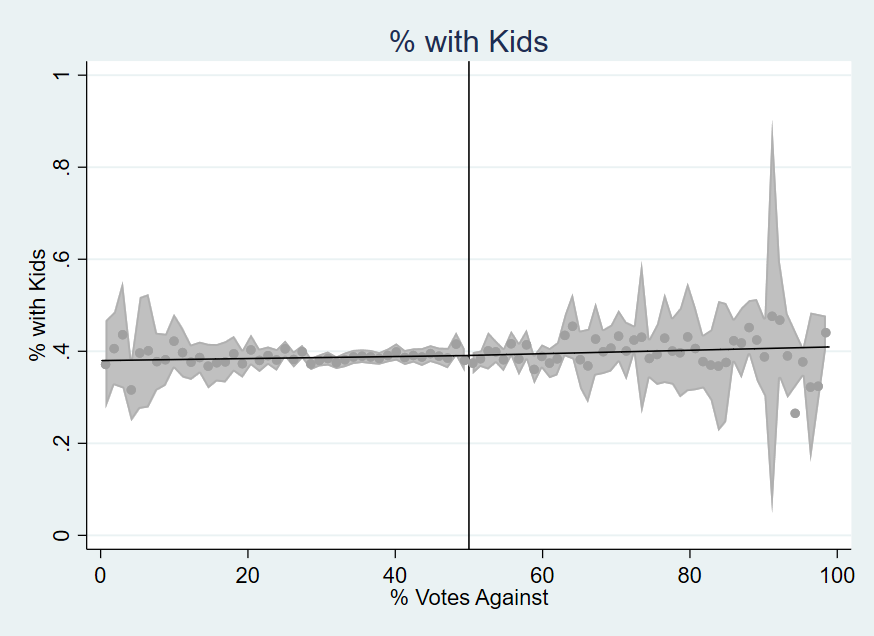
\includegraphics[width=\textwidth,keepaspectratio]{images/cov_smoothness_pctwithkids.png}
            % \caption{Year 3 after vote}
            \label{fig:pct_with_kids_sm}
        \end{subfigure}
    \end{minipage}
    \hfill
    \begin{minipage}[b]{0.48\textwidth}
        \centering
        \begin{subfigure}[b]{\textwidth}
            \centering
            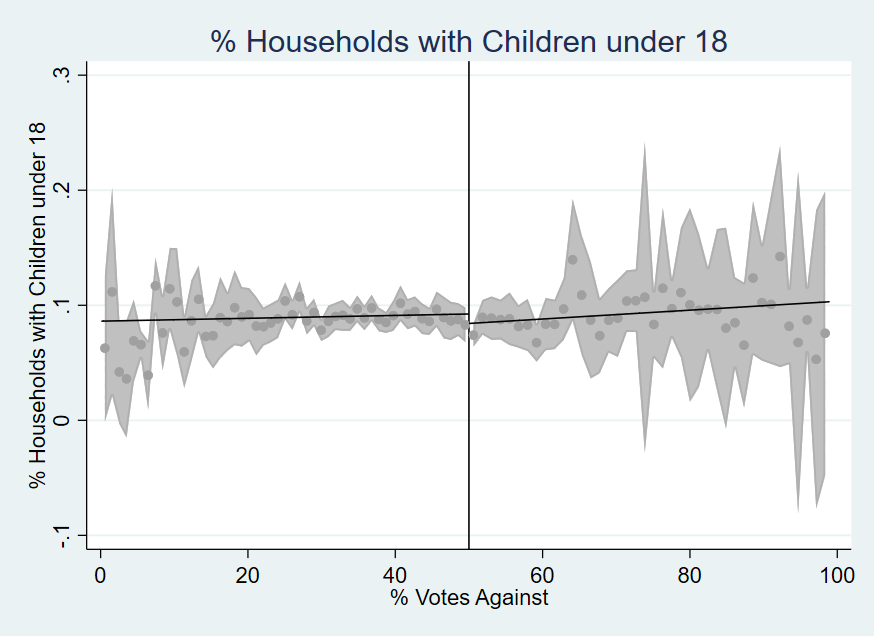
\includegraphics[width=\textwidth,keepaspectratio]{images/cov_smoothness_pctsinparhhld.png}
            % \caption{Year 4 after vote}
            \label{fig:pctsinparhhld_sm}
        \end{subfigure}
    \end{minipage}

    \vspace{1em}

    \begin{minipage}[b]{0.48\textwidth}
        \centering
        \begin{subfigure}[b]{\textwidth}
            \centering
            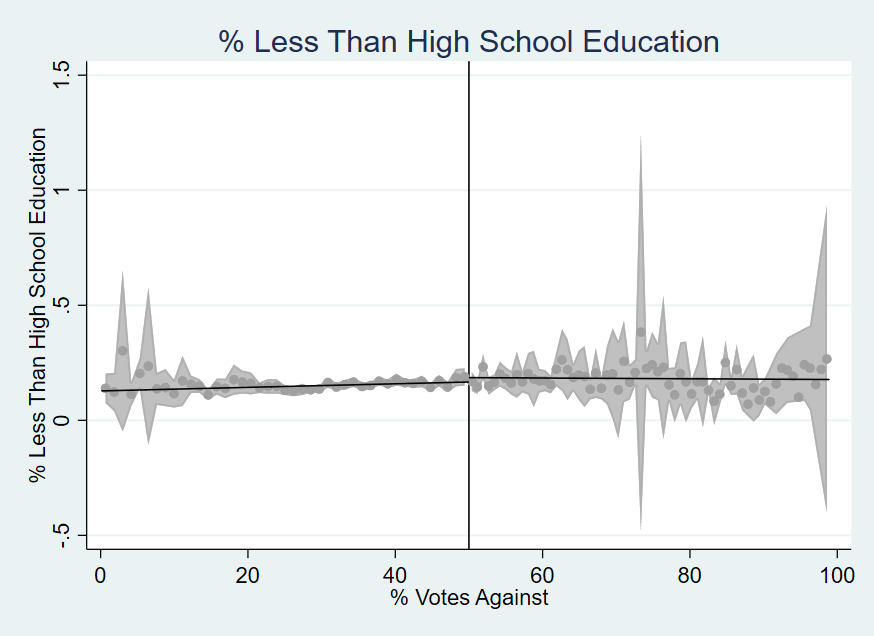
\includegraphics[width=\textwidth,keepaspectratio]{images/cov_smoothness_pctlesshs.png}
            % \caption{Year 5 after vote}
            \label{fig:pctlesshs_sm}
        \end{subfigure}
    \end{minipage}
    \hfill
    \begin{minipage}[b]{0.48\textwidth}
        \centering
        \begin{subfigure}[b]{\textwidth}
            \centering
            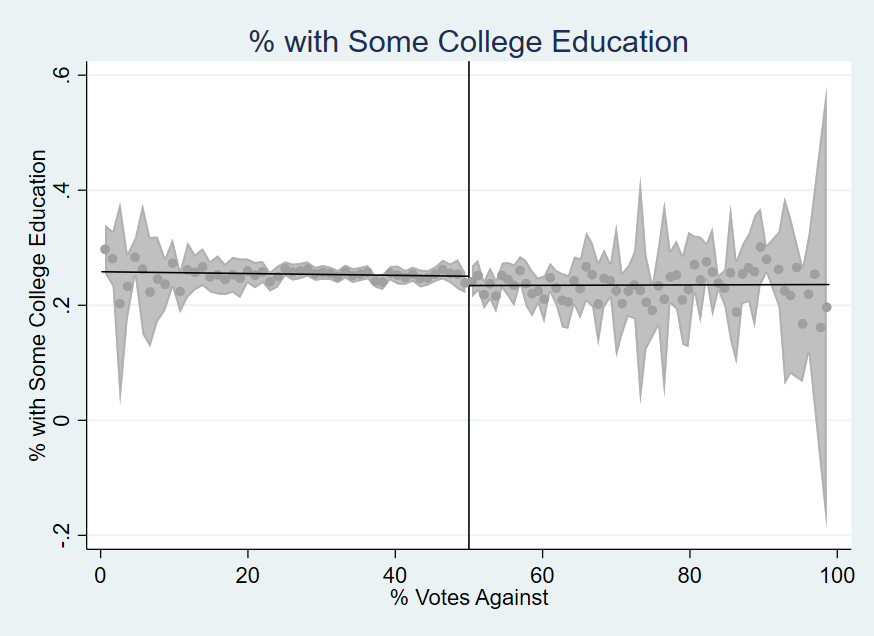
\includegraphics[width=\textwidth,keepaspectratio]{images/cov_smoothness_pctsomecoll.png}
            % \caption{Year 6 after vote}
            \label{fig:pctsomecoll_sm}
        \end{subfigure}
    \end{minipage}    

    \vspace{1em}

    \begin{minipage}[b]{0.48\textwidth}
        \centering
        \begin{subfigure}[b]{\textwidth}
            \centering
            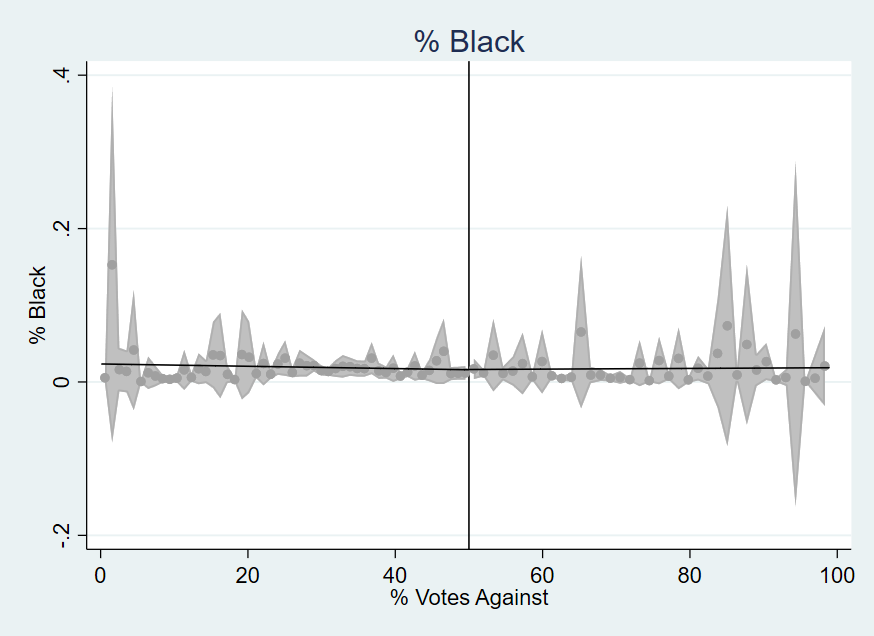
\includegraphics[width=\textwidth,keepaspectratio]{images/cov_smoothness_pctblack.png}
            % \caption{Year 7 after vote}
            \label{fig:black_sm}
        \end{subfigure}
    \end{minipage}
    \hfill
    \begin{minipage}[b]{0.48\textwidth}
        \centering
        \begin{subfigure}[b]{\textwidth}
            \centering
            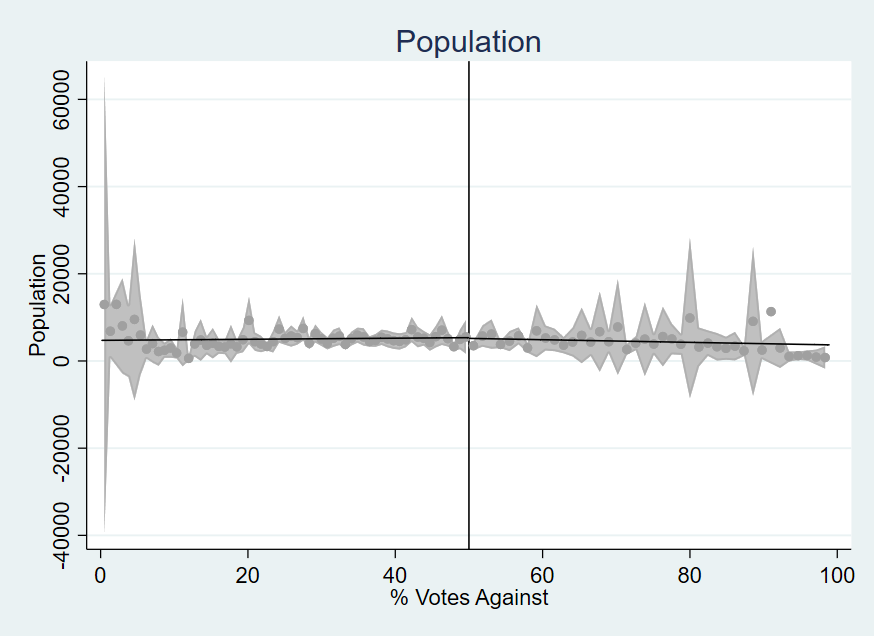
\includegraphics[width=\textwidth,keepaspectratio]{images/cov_smoothness_pop.png}
            % \caption{Year 8 after vote}
            \label{fig:pop_sm}
        \end{subfigure}
    \end{minipage}        

    % \vspace{1em}

    \caption{Covariate Discontinuity Plots - Part 1}
    \label{fig:rd_cov_smoothness_1}
\end{figure}

\begin{figure}[ht]
    \centering
    \begin{minipage}[b]{0.48\textwidth}
        \centering
        \begin{subfigure}[b]{\textwidth}
            \centering
            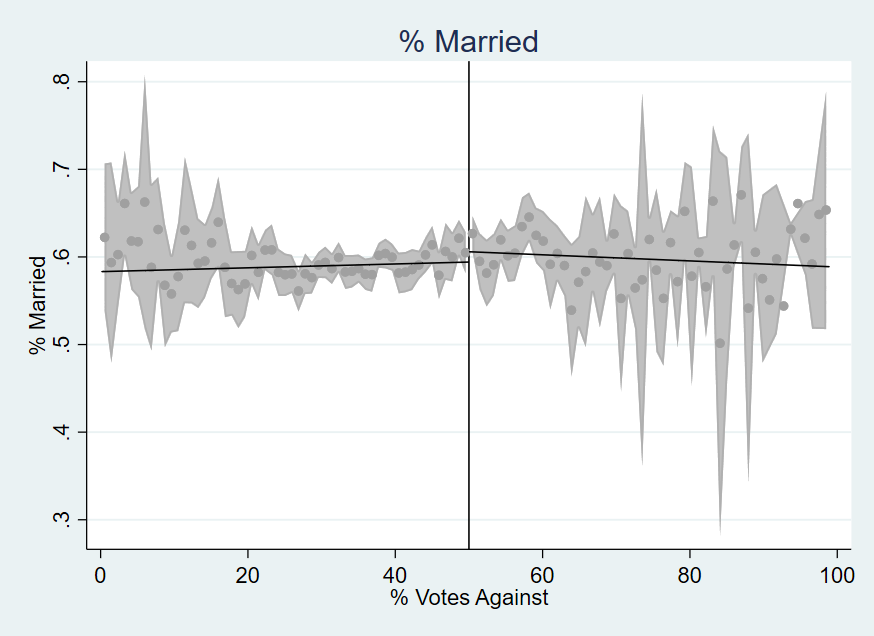
\includegraphics[width=\textwidth,keepaspectratio]{images/cov_smoothness_pctmarried.png}
            \label{fig:pctmarried_sm}
        \end{subfigure}
    \end{minipage}
    \hfill
    \begin{minipage}[b]{0.48\textwidth}
        \centering
        \begin{subfigure}[b]{\textwidth}
            \centering
            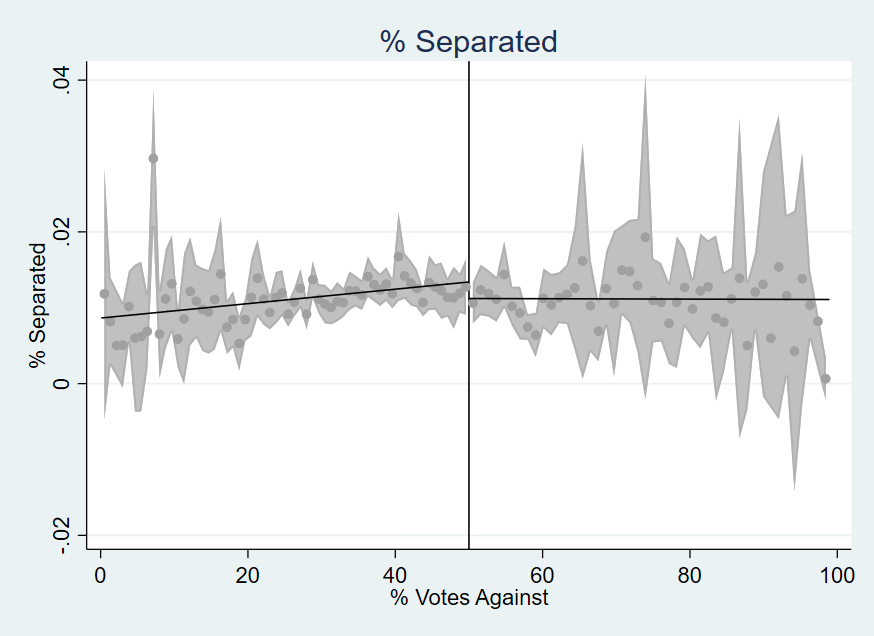
\includegraphics[width=\textwidth,keepaspectratio]{images/cov_smoothness_pctseparated.png}
            \label{fig:pctseparated_sm}
        \end{subfigure}
    \end{minipage}

    \vspace{1em}

    \begin{minipage}[b]{0.48\textwidth}
        \centering
        \begin{subfigure}[b]{\textwidth}
            \centering
            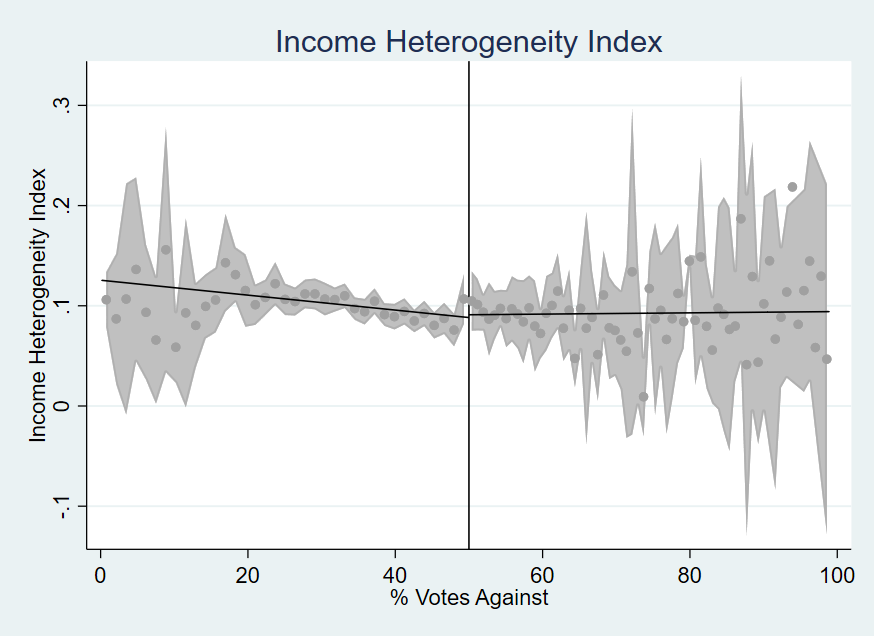
\includegraphics[width=\textwidth,keepaspectratio]{images/cov_smoothness_incherfindahl.png}
            \label{fig:incherfindahl_sm}
        \end{subfigure}
    \end{minipage}
    \hfill
    \begin{minipage}[b]{0.48\textwidth}
        \centering
        \begin{subfigure}[b]{\textwidth}
            \centering
            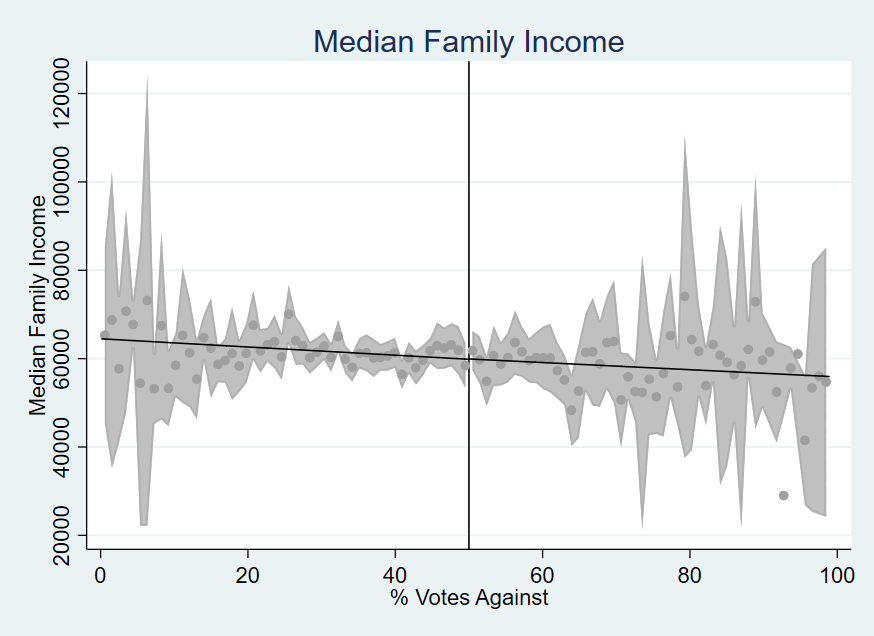
\includegraphics[width=\textwidth,keepaspectratio]{images/cov_smoothness_medfamy.png}
            \label{fig:medfamy_sm}
        \end{subfigure}
    \end{minipage}

    \vspace{1em}

    \begin{minipage}[b]{0.48\textwidth}
        \centering
        \begin{subfigure}[b]{\textwidth}
            \centering
            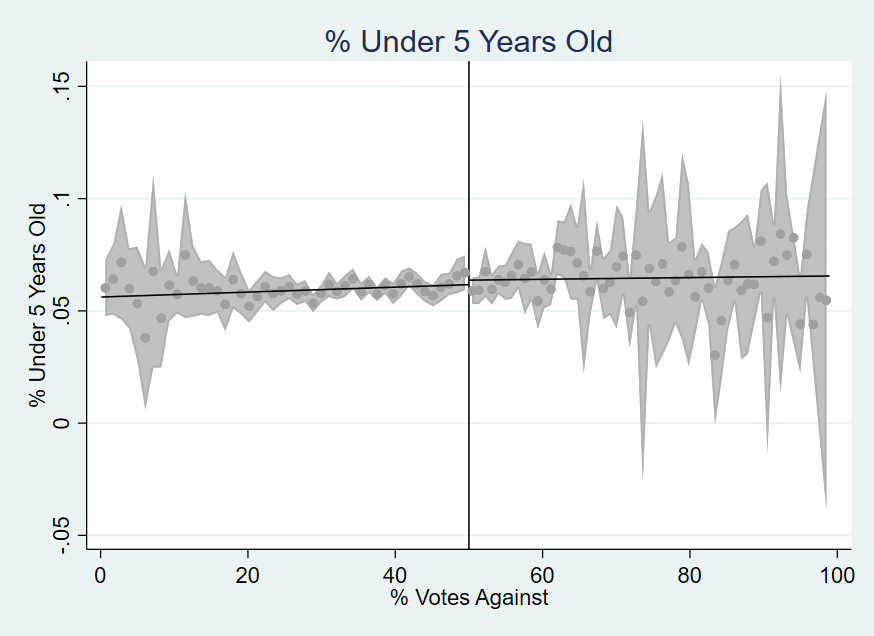
\includegraphics[width=\textwidth,keepaspectratio]{images/cov_smoothness_pctlt5.png}
            \label{fig:pctlt5_sm}
        \end{subfigure}
    \end{minipage}
    \hfill
    \begin{minipage}[b]{0.48\textwidth}
        \centering
        \begin{subfigure}[b]{\textwidth}
            \centering
            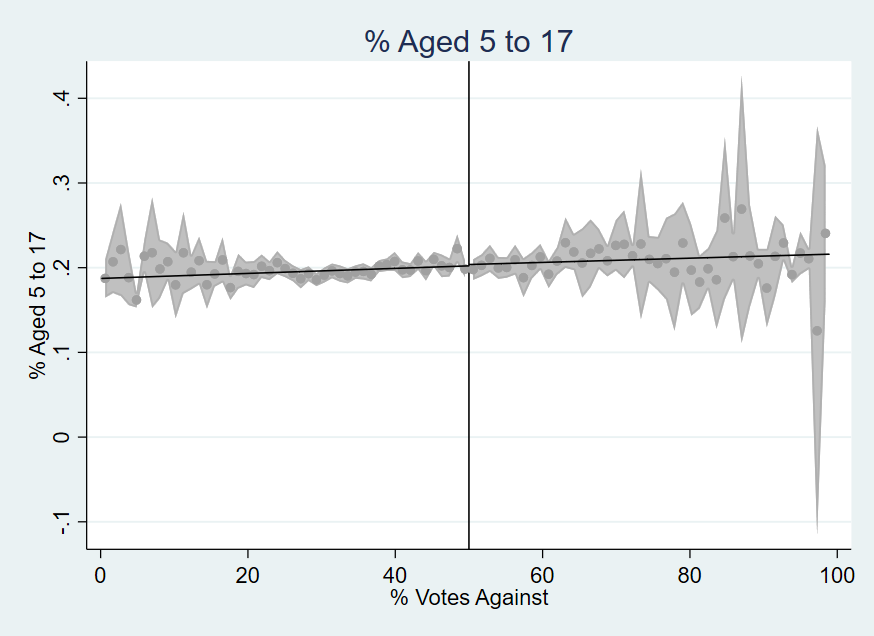
\includegraphics[width=\textwidth,keepaspectratio]{images/cov_smoothness_pct5to17.png}
            \label{fig:pct5to17_sm}
        \end{subfigure}
    \end{minipage}    

    \vspace{1em}

    \begin{minipage}[b]{0.48\textwidth}
        \centering
        \begin{subfigure}[b]{\textwidth}
            \centering
            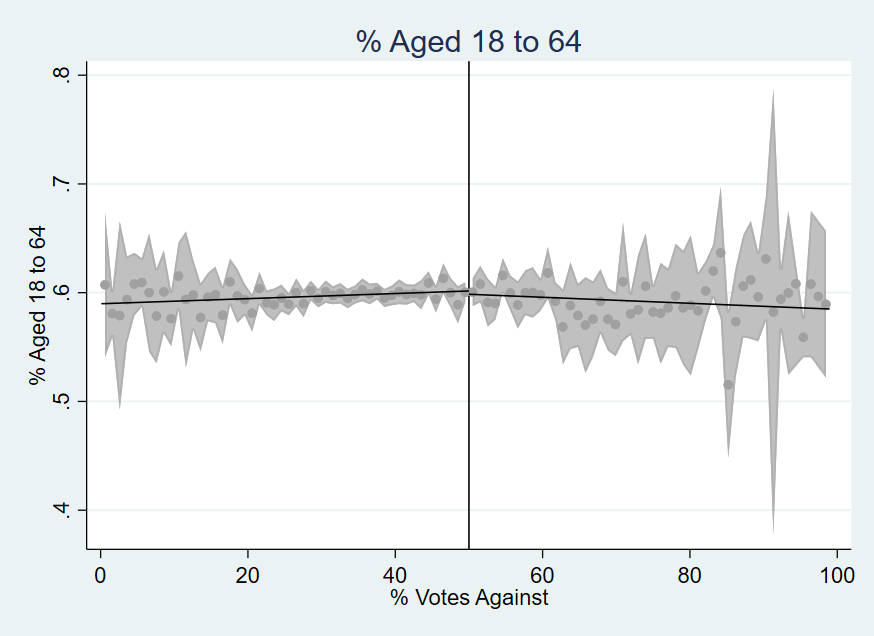
\includegraphics[width=\textwidth,keepaspectratio]{images/cov_smoothness_pct18to64.png}
            \label{fig:pct18to64_sm}
        \end{subfigure}
    \end{minipage}
    \hfill
    \begin{minipage}[b]{0.48\textwidth}
        \centering
        \begin{subfigure}[b]{\textwidth}
            \centering
            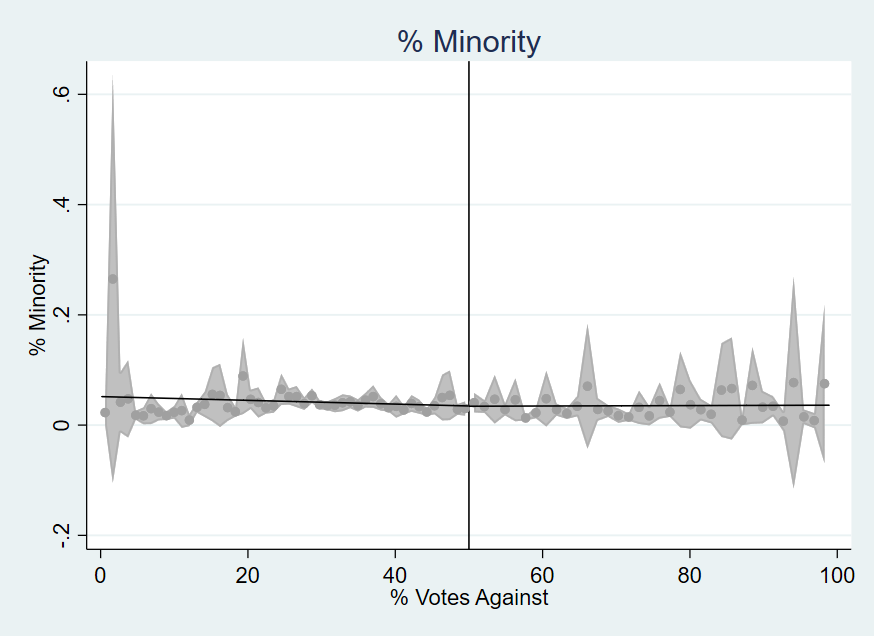
\includegraphics[width=\textwidth,keepaspectratio]{images/cov_smoothness_pctmin.png}
            \label{fig:pctmin_sm}
        \end{subfigure}
    \end{minipage}        

    % \vspace{1em}

    \caption{Covariate Discontinuity Plots - Part 2}
    \label{fig:rd_cov_smoothness_2}
\end{figure}


\clearpage

\subsection{Covariate Discontinuity Tests}

\begin{table}[!h]
    \centering
    \caption{Covariate Discontinuity Test Results}
    \label{tab:covariate_discontinuity}
    \begin{tabular}{p{2cm}cccc}
        \hline
        Variable & Estimate & Standard error & p-value & Confidence interval \\
        \hline
        Population                           & -388      & 1,094   & 0.722  & [-2,532, 1,755] \\
        Poverty Rate                         & 0.017     & 0.014   & 0.234  & [-0.011, 0.045] \\
        \% with Kids                         & -0.007    & 0.012   & 0.539  & [-0.030, 0.015] \\
        \% Households with Children under 18 & 0.0001    & 0.007   & 0.981  & [-0.014, 0.014] \\
        \% Less than High School Education   & -0.004    & 0.020   & 0.834  & [-0.043, 0.035] \\
        \% Some College Education            & -0.012    & 0.011   & 0.274  & [-0.034, 0.009] \\
        \% Unemployment Rate                 & -0.002    & 0.006   & 0.733  & [-0.013, 0.009] \\
        \% Renters                           & -0.005    & 0.015   & 0.754  & [-0.035, 0.025] \\
        \% White                             & -0.007    & 0.011   & 0.499  & [-0.028, 0.014] \\
        \% Black                             & -0.004    & 0.009   & 0.685  & [-0.021, 0.014] \\
        \% Married                           & -0.013    & 0.015   & 0.374  & [-0.042, 0.016] \\
        \% Separated                         & 0.001     & 0.002   & 0.485  & [-0.002, 0.004] \\
        \hline
    \end{tabular}
    \begin{tablenotes}
        \small
        \item Estimates indicate the treatment effect of failing to renew a road maintenance tax levy on each covariate considered during our study. Confidence intervals are presented in square brackets.
    \end{tablenotes}
\end{table}

\begin{table}[!h]
    \centering
    \caption{Covariate means for high-poverty sample used in wage outcome regressions}
    \label{tab:covariate_means_wage}
    \begin{tabular}{p{4cm}cc}
        \hline
        Covariate & Failed levies & Passed levies \\
        \hline
        \% Black                & 0.03  & 0.03  \\
        \% Married              & 0.55  & 0.53  \\
        \% Unemployment Rate    & 0.073 & 0.075 \\
        \% Renters              & 0.26  & 0.27  \\
        \% Aged 5 to 17         & 0.22  & 0.21  \\
        Population              & 3,398 & 4,465 \\
        Labor Force Participation & 0.59  & 0.58  \\
        \% Aged 65+             & 0.13  & 0.14  \\
        \% with Kids            & 0.41  & 0.41  \\
        \% Some College Education & 0.21  & 0.23  \\
        \% Bachelors Degree     & 0.06  & 0.07  \\
        \% Hispanic             & 0.01  & 0.01  \\
        Number of Observations  & 83    & 296   \\
        \hline
    \end{tabular}
    \begin{tablenotes}
        \small
        \item Covariate means for High-Poverty sample regressions using the natural log of Wages as the outcome variable corresponding to Table \ref{tab:wages_per_worker}. Covariate means shown for an effective bandwidth of h = 0.14 at the time of the vote for the set of cities that renew or cut road tax levies. The authors suggest the only sizable difference is Population. The danger for identification is that Population differences may be driving tax levy renewal, but we find the correlation is only 0.07.
    \end{tablenotes}
\end{table}

\clearpage

\section{Appendix C: Additional Information} \label{sec:appxc}

\subsection{Roads in Waynesville OH: Serial Cutter of Road Maintenance Tax Levies}

% \begin{figure}[htbp]
%     \centering
%     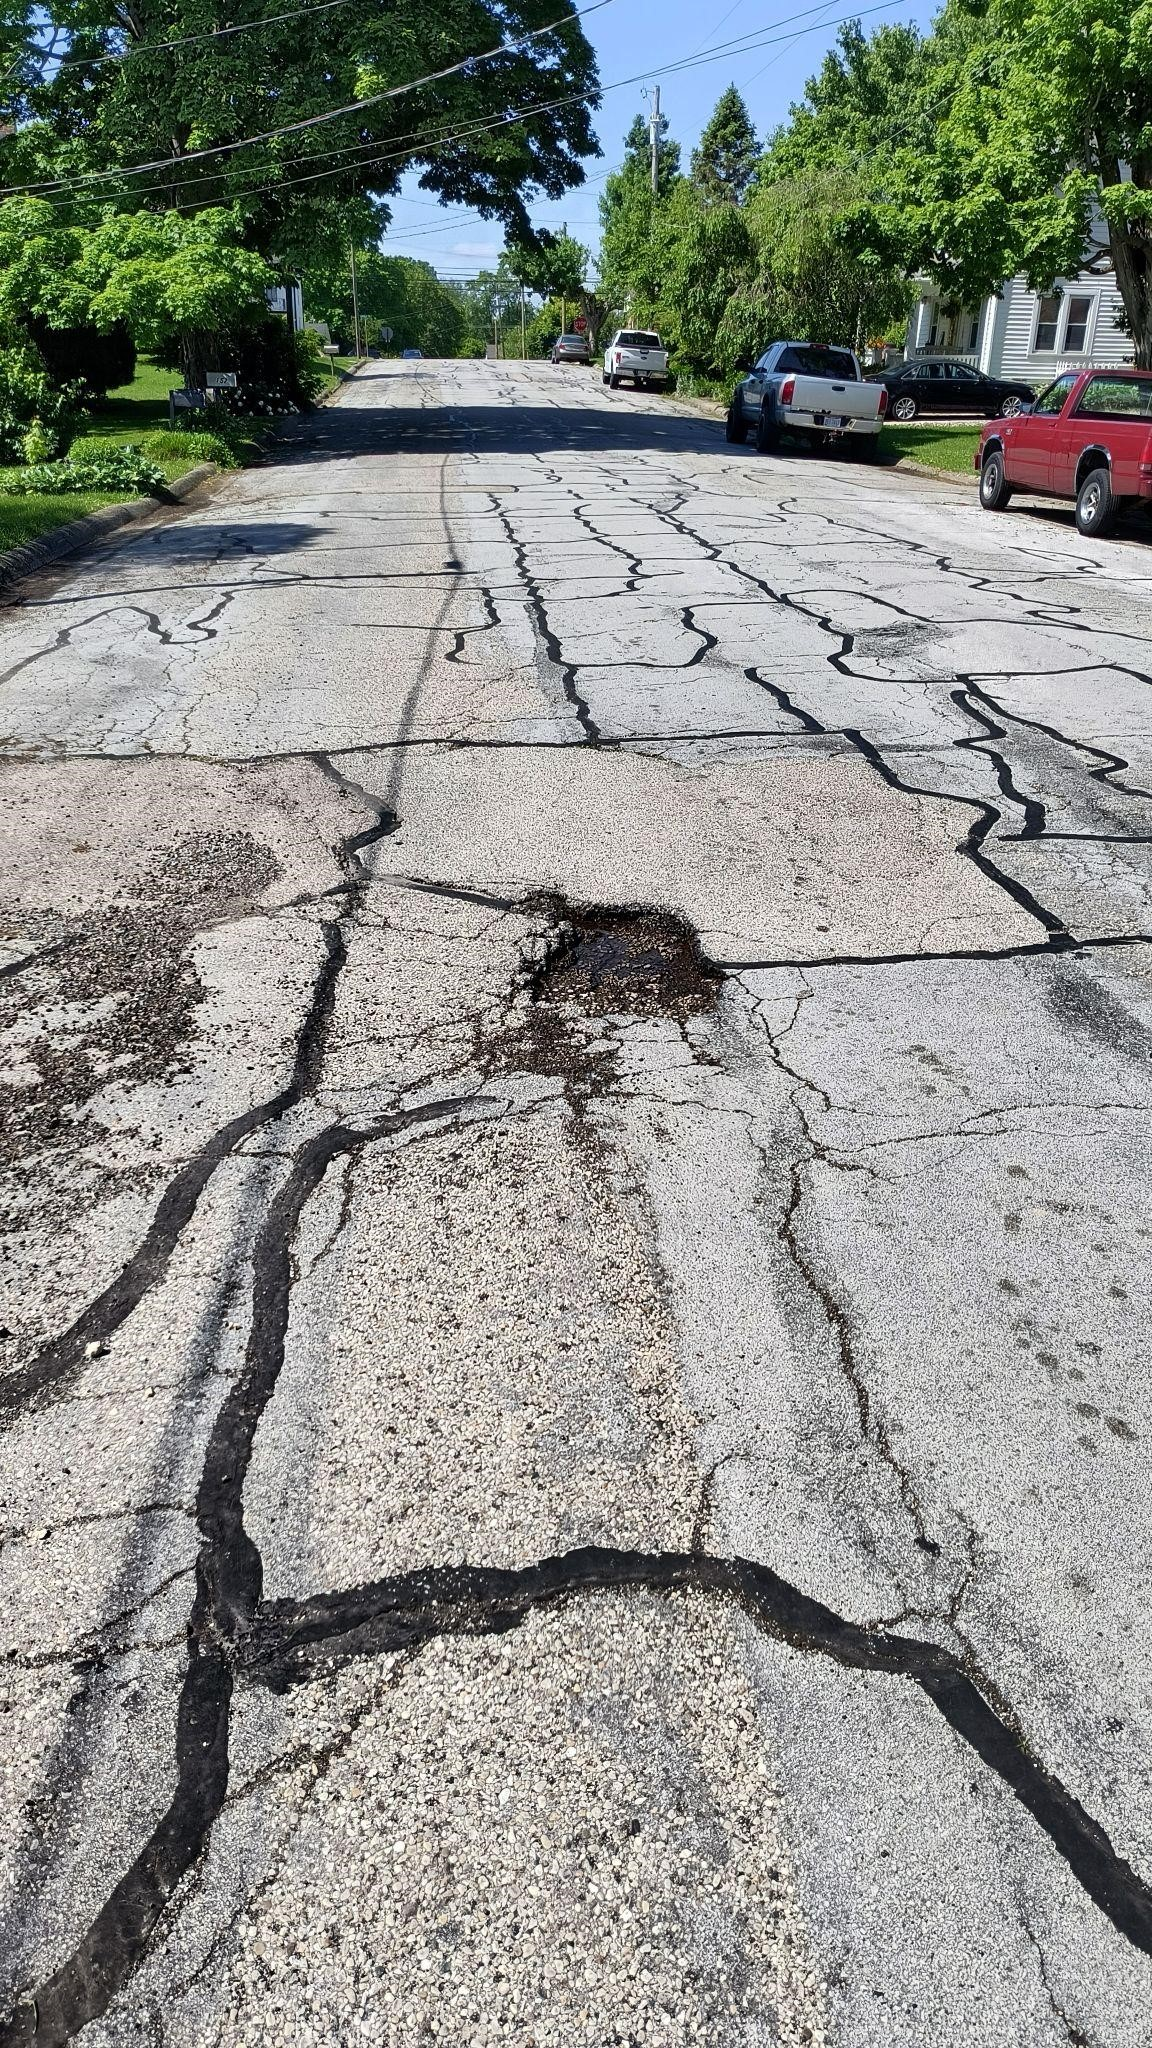
\includegraphics[width=\textwidth,keepaspectratio]{images/waynesville_oh_1.png}
%     \label{fig:w_oh_1}
% \end{figure}

\begin{figure}[ht]
    \centering
    \begin{minipage}[b]{0.48\textwidth}
        \centering
        \begin{subfigure}[b]{0.75\textwidth}  % Change 1: Reduced to 75% width
            \centering
            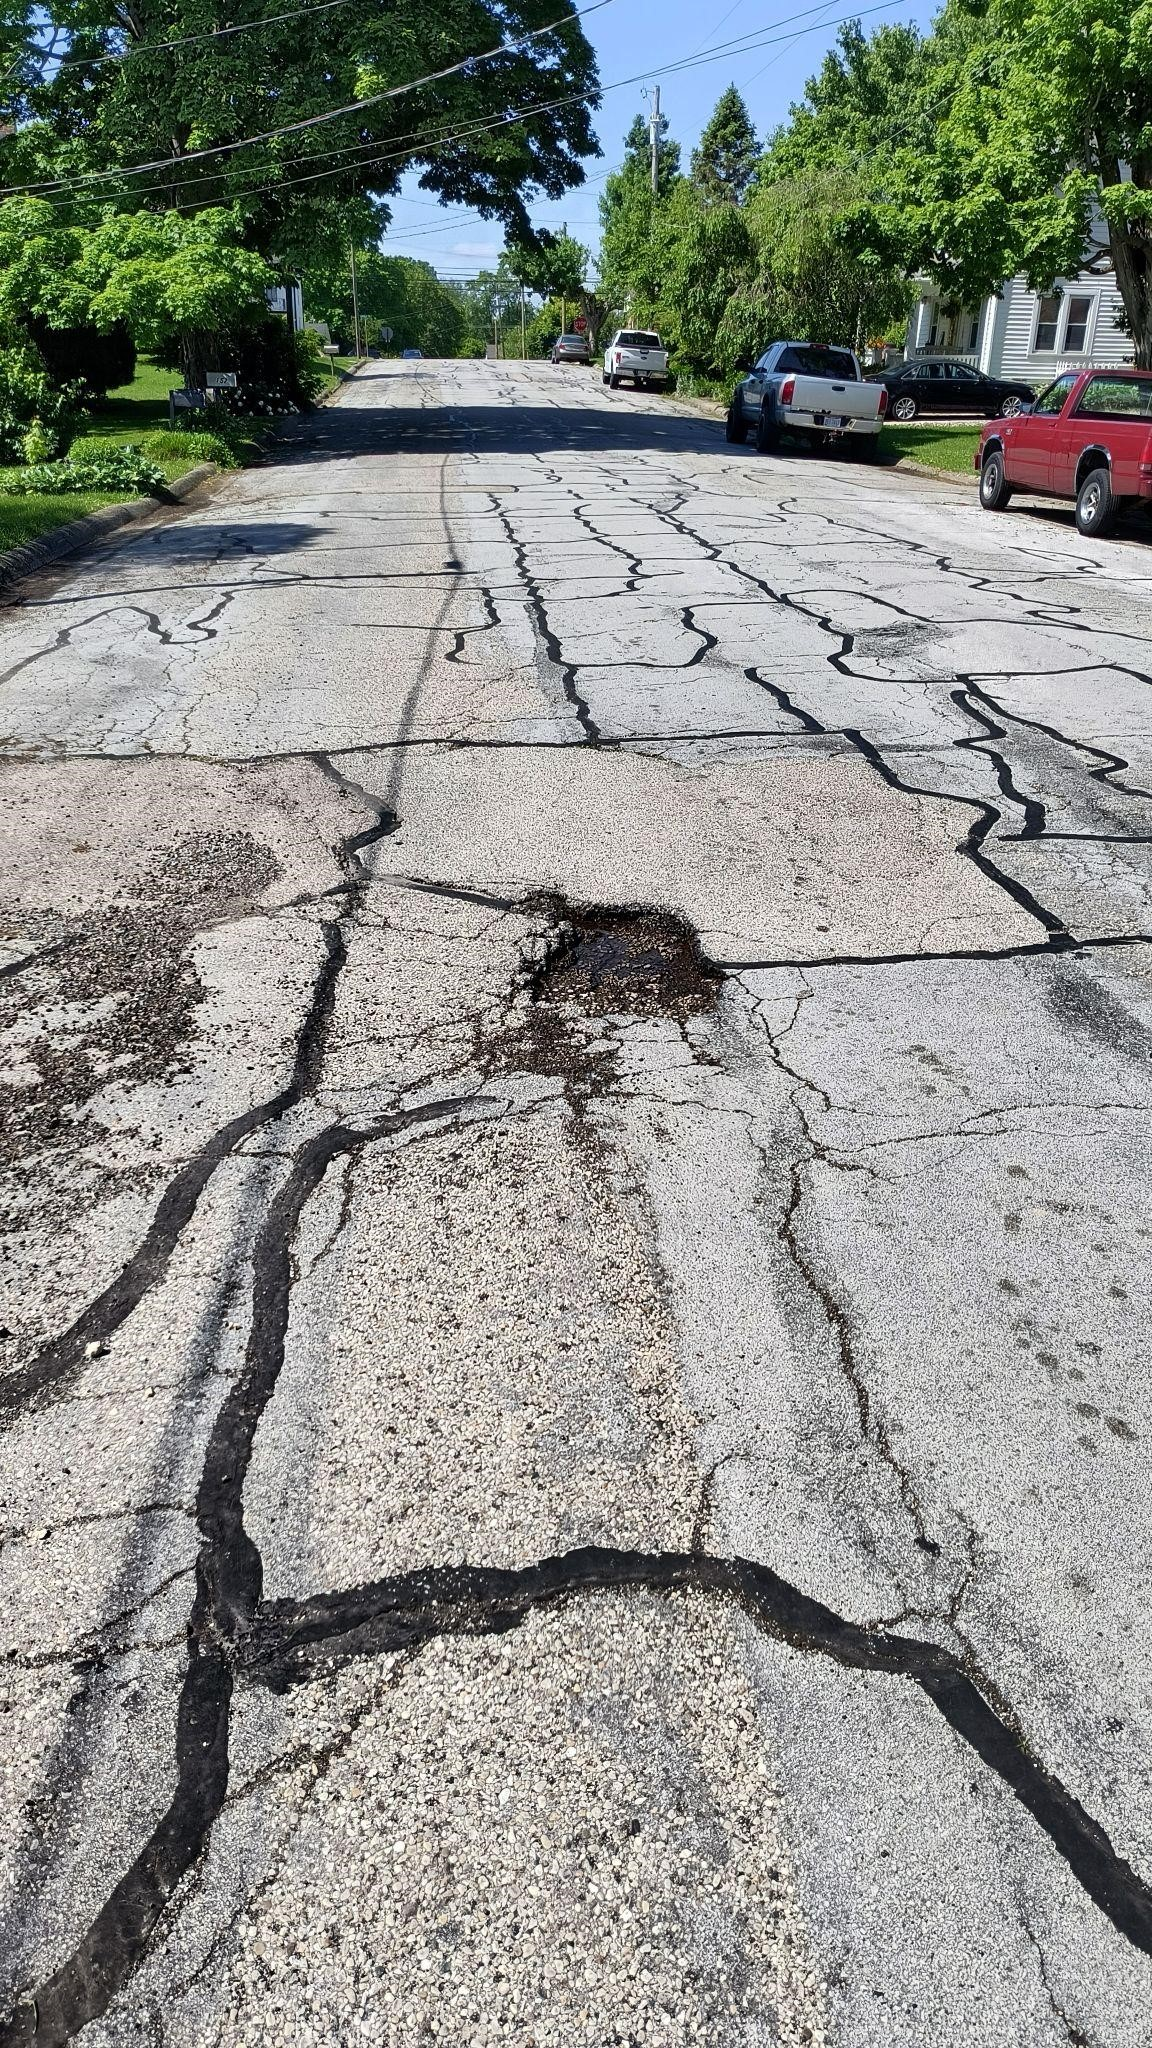
\includegraphics[width=\textwidth,keepaspectratio]{images/waynesville_oh_1.png}
            \label{fig:w_oh_1}
        \end{subfigure}
    \end{minipage}
    \hfill
    \begin{minipage}[b]{0.48\textwidth}
        \centering
        \begin{subfigure}[b]{0.75\textwidth}  % Change 2: Reduced to 75% width
            \centering
            \includegraphics[width=\textwidth,keepaspectratio]{images/waynesville_oh_2.png}
            \label{fig:w_oh_2}
        \end{subfigure}
    \end{minipage}

    \vspace{1em}

    \begin{minipage}[b]{0.48\textwidth}
        \centering
        \begin{subfigure}[b]{0.75\textwidth}  % Change 3: Reduced to 75% width
            \centering
            \includegraphics[width=\textwidth,keepaspectratio]{images/waynesville_oh_3.png}
            \label{fig:w_oh_3}
        \end{subfigure}
    \end{minipage}

    \caption{Roads in Waynesville: Case Study}
    \label{fig:rd_waynesville}
\end{figure}


\end{document}